\input{../style/preamble}
\input{../latex-math/basic-math}
\input{../latex-math/basic-ml}
\input{../latex-math/ml-nn}

% Macros used by the adapted DL4NLP source material, not present in this course's own
% preamble (same set added in sessions 7-8; kept in sync here).
\newcommand{\ques}{\textbf{\textcolor{red}{Question:  }}}
\newcommand{\myblue}[1]{\textcolor{blue}{#1}}
\newcommand{\citebutton}[2]{\beamergotobutton{\href{#2}{#1}}}
\newcommand\warning{%
 \makebox[1.4em][c]{%
 \makebox[0pt][c]{\raisebox{.1em}{\scriptsize!}}%
 \makebox[0pt][c]{\color{red}\normalsize$\bigtriangleup$}}}%

\newcommand{\titlefigure}{figure/twotypesoflearning.png}
\newcommand{\learninggoals}{
  \item Complete the three-Transformer-families taxonomy: GPT-1 $\to$ GPT-2 $\to$ GPT-3 as the decoder-only flagship, and how the recipe scaled into in-context learning
  \item Precise terminology for fine-tuning and prompting: single-task, multi-task, few-shot, instruction tuning
  \item Chain-of-thought reasoning and why bigger models reason better -- and DeepSeek-R1, where reasoning is trained via automatic, verifiable rewards instead
  \item What it actually costs to train an LLM: compute, memory, distributed training, FlashAttention
  \item Scaling laws: Kaplan vs.\ Chinchilla, and whether scaling has plateaued
}

\title{Advanced Artificial Intelligence and Machine Learning}
\date{}

\begin{document}

\lecturechapter{Large Language Models}
\lecture{Advanced AI \& ML}
%%%%%%%%%%%%%%%%%%%%%%%%%%%%%%%%%%%%%%%%%%%%%%%%%%%%%%%%%%%%%%%%%%

\section{Recap: The Decoder-Only Family}
%%%%%%%%%%%%%%%%%%%%%%%%%%%%%%%%%%%%%%%%%%%%%%%%%%%%%%%%%%%%%%%%%%

\begin{vbframe}{Completing the Taxonomy}
\begin{itemize}
  \item Sessions 7 and 8 introduced the three Transformer families and went deep on encoder-only (BERT) and encoder-decoder (T5) models, naming GPT as ``session 9's subject'' every time the decoder-only column came up.
\end{itemize}
\begin{center}
\footnotesize
\begin{tabular}{@{}p{2.1cm}p{2.8cm}p{2.6cm}p{3.2cm}@{}}
\toprule
 & \textbf{Encoder-only} & \textbf{Decoder-only} & \textbf{Encoder-decoder} \\
\midrule
Attention & bidirectional & causal (masked) & both (+ cross-attn.) \\[2pt]
Pretraining obj. & masked LM & next-token & varies (e.g.\ span corruption) \\[2pt]
Typical use & understanding, embedding & generation & sequence-to-sequence \\[2pt]
Flagship model & BERT & \textbf{GPT (today)} & original Transformer, T5 \\
\bottomrule
\end{tabular}
\end{center}
\begin{itemize}
  \item This session closes the loop: GPT-1 through GPT-3 as the decoder-only family's evolution, then everything that turns a raw next-token predictor into something you can actually use -- fine-tuning, prompting, chain-of-thought reasoning -- and what it costs to train and scale one.
\end{itemize}
\end{vbframe}

%%%%%%%%%%%%%%%%%%%%%%%%%%%%%%%%%%%%%%%%%%%%%%%%%%%%%%%%%%%%%%%%%%

\section{GPT-1: The Original Recipe}
%%%%%%%%%%%%%%%%%%%%%%%%%%%%%%%%%%%%%%%%%%%%%%%%%%%%%%%%%%%%%%%%%%

\begin{vbframe}{GPT-1: Generative Pre-Training}
\begin{figure}
\centering
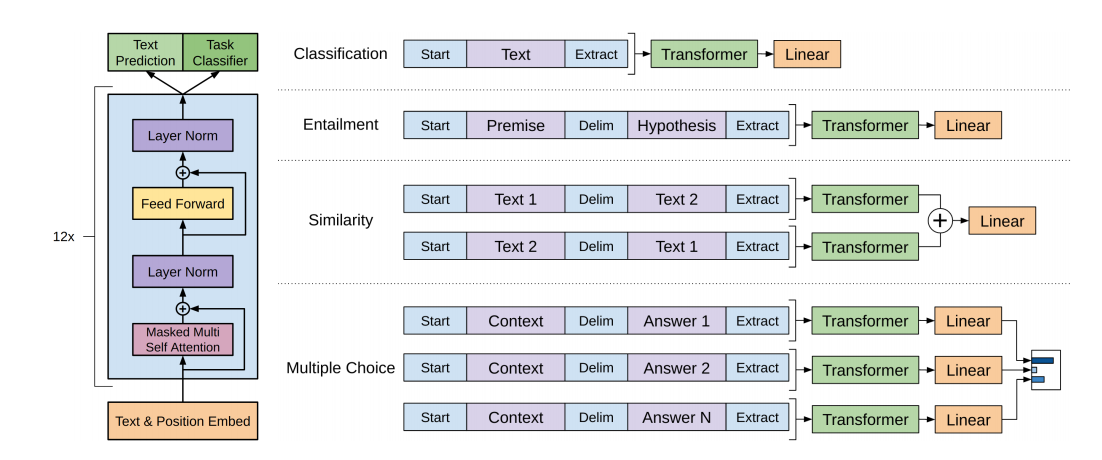
\includegraphics[width=.75\textwidth]{figure/71-gpt.png}\\
\citebutton{Source: Radford et al., 2018}{https://openai.com/blog/language-unsupervised/}
\end{figure}
\begin{itemize}
  \item Radford et al.\ (2018): pretrain a Transformer \textbf{decoder} on unlabeled text with a standard language-modeling objective, then fine-tune on a labeled downstream task.
  \item The same two-stage recipe as BERT (session 8) -- but the backbone is a decoder, not an encoder, so the model is generative from the start.
\end{itemize}
\end{vbframe}

\begin{vbframe}{GPT-1: Architectural Details}
\begin{itemize}
  \item Transformer \textit{decoder} as backbone, 12 layers, masked (causal) self-attention
  \item Hidden dimension $H=768$, $A=12$ attention heads
  \item BPE vocabulary with 40k merges (recall session 7's tokenization section)
  \item \textit{Learned} positional embeddings, not the fixed sinusoidal ones of the original Transformer
\end{itemize}
With $U=(w_{t-k},\ldots,w_{t-1})$:
\begin{align*}
  \vec h_0 &= \vec U \vec W_e + \vec W_p \\
  \vec h_l &= \text{Trafo}(\vec h_{l-1}) \quad \forall l \in [1,n]\\
  P(w_t) &= \text{softmax}(\vec h_n \vec W_e^\top)
\end{align*}
\end{vbframe}

\begin{vbframe}{Pre-Training and Fine-Tuning GPT-1}
\textbf{Pre-training} -- standard LM objective on an \textit{unlabeled} sequence:
$$L_1(\{w_1,\ldots,w_n\}) = \sum_i \log P(w_t \mid w_{t-k},\ldots,w_{t-1};\Theta)$$
\begin{itemize}
  \item \textit{Resource:} BooksCorpus, $>$7k unpublished books -- long, coherent texts that let the model learn long-range dependencies.
\end{itemize}
\textbf{Fine-tuning} -- a linear+softmax head on top, plus an auxiliary LM term ($L_3 = L_2 + \lambda L_1$) that speeds convergence and improves generalization. Task-specific \textit{input transformations} let one architecture handle many tasks without new modules: entailment concatenates premise and hypothesis ($[p;\$;h]$), similarity uses both orderings, QA concatenates context, question, and each candidate answer. Fine-tuning itself is quick -- 3 epochs sufficed.
\end{vbframe}

\begin{vbframe}{GPT-1 Parameter Count}
\begin{itemize}
  \item \textbf{We know:} $n_{layers}=12$, $d_{model}=768$, $V=40{,}000$, $M=512$ (max sequence length)
  \item \textbf{Also:} $N_{Decoder} = 12\cdot d_{model}^2$ (note: \textit{not} $16\cdot d_{model}^2$, since a decoder-only stack has no cross-attention -- unlike T5's decoder in session 8), and\\
  $N_{Embedding} = \underbrace{V\times d_{model}}_{\text{token emb.}} + \underbrace{M\times d_{model}}_{\text{pos.\ emb.}}$
\end{itemize}
$$
N_{total} = n_{layers}\cdot N_{Decoder} + N_{Embedding} = 12\cdot 12\cdot 768^2 + 40{,}000\times 768 + 512\times 768 \approx 117\text{M}
$$
\begin{itemize}
  \item The same style of derivation as BERT's and T5's parameter counts in session 8 -- worth comparing all three side by side.
\end{itemize}
\end{vbframe}

%%%%%%%%%%%%%%%%%%%%%%%%%%%%%%%%%%%%%%%%%%%%%%%%%%%%%%%%%%%%%%%%%%

\section{GPT-2: Language Models as Multitask Learners}
%%%%%%%%%%%%%%%%%%%%%%%%%%%%%%%%%%%%%%%%%%%%%%%%%%%%%%%%%%%%%%%%%%

\begin{vbframe}{GPT-2: Scale and a New Corpus}
\begin{itemize}
  \item Radford et al.\ (2019) -- same decoder-only recipe, but bigger and trained differently: a custom web scrape of all outbound Reddit links (8M documents, 40GB of text), byte-level BPE, context length doubled ($512\to1024$).
  \item Released in four sizes, up to 1.5B parameters ($\sim$13$\times$ GPT-1) -- the first time this course sees ``just scale it up'' as an explicit strategy in its own right.
  \item \citebutton{Source: Radford et al., 2019}{https://openai.com/research/better-language-models}
\end{itemize}
\end{vbframe}

\begin{vbframe}{Capabilities: Storytelling (and Hallucination)}
\begin{figure}
\centering
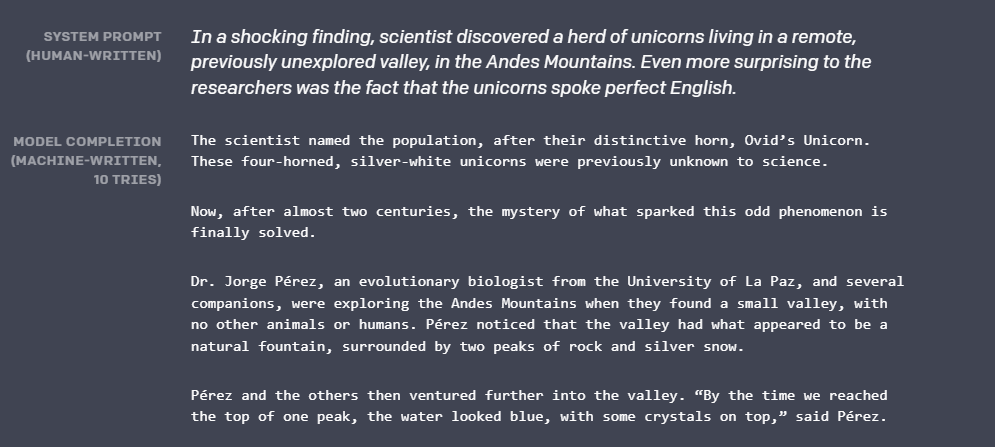
\includegraphics[width=.55\textwidth]{figure/72-gpt2-story.png}\\
\citebutton{Source: OpenAI Blog}{https://openai.com/research/better-language-models}
\end{figure}
\begin{itemize}
  \item In 2019: a striking achievement -- the model continues a made-up story \textit{coherently}, inventing its own consistent facts (``four-horned\ldots unicorns'').
  \item Still not fully consistent. What was called a quirky curiosity in 2019 is exactly what we now call \textbf{hallucination} -- a problem still unsolved today, and the target of substantial ongoing research.
\end{itemize}
\end{vbframe}

\begin{vbframe}{Language Models as Multitask Learners}
\begin{itemize}
  \item Core idea: ``language provides a flexible way to specify tasks, inputs, and outputs all as a sequence of symbols'' -- a translation example is just the sequence (\textit{translate to french, english text, french text}).
  \item The model benefits from seeing \textit{natural} occurrences of task demonstrations during pretraining on large web corpora -- no explicit task-specific fine-tuning required.
  \item Related rationale to T5's text-to-text reframing (session 8), but different in \textit{when} the task format is learned: T5 learns literal task prefixes during supervised fine-tuning; GPT-2 picks this up incidentally, already during pretraining.
\end{itemize}
\end{vbframe}

\begin{vbframe}{Capabilities: Zero-Shot}
\begin{figure}
\centering
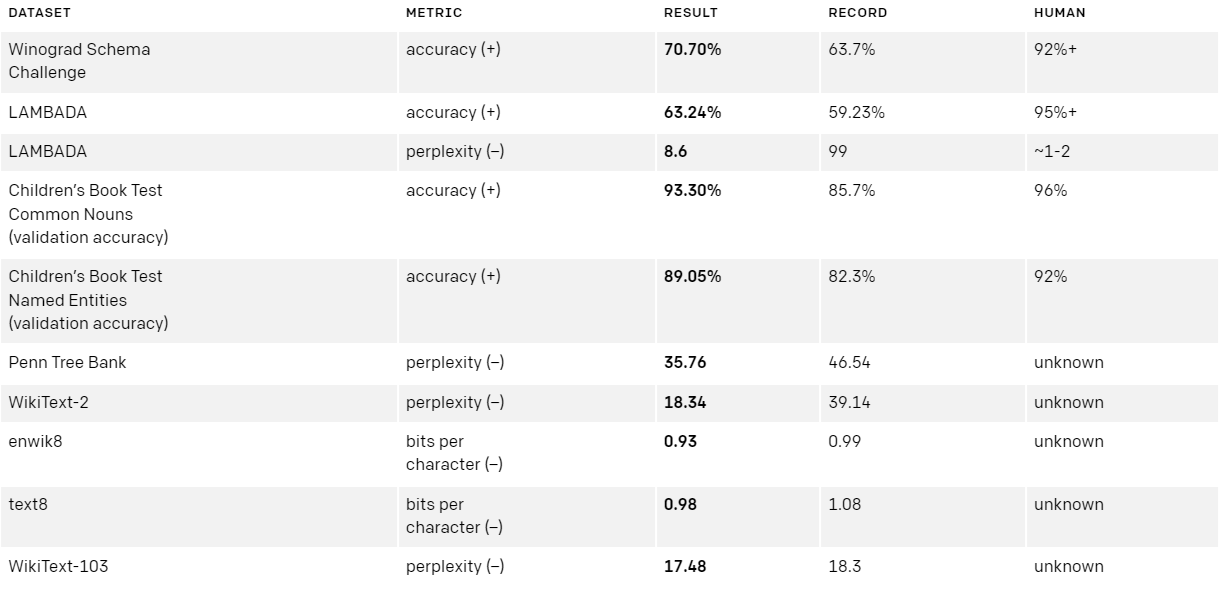
\includegraphics[width=.85\textwidth]{figure/72-gpt2-zeroshot.png}\\
\citebutton{Source: Radford et al., 2019}{https://openai.com/research/better-language-models}
\end{figure}
\begin{itemize}
  \item \textbf{Zero-shot:} solve a task the model was never explicitly trained on, given only a description of the task -- no input/output demonstrations.
  \item \textbf{Few-shot} relaxes this: also provide demonstrations, but still \textit{no} gradient updates.
  \item This distinction, demonstrated here on a range of tasks, paves the way directly to GPT-3.
\end{itemize}
\end{vbframe}

\begin{vbframe}{Capabilities: Factual Knowledge and Scale}
\textbf{Natural Questions} \citebutton{Kwiatkowski et al., 2019}{https://aclanthology.org/Q19-1026/} -- testing factual knowledge stored implicitly in the pretrained weights:
\begin{itemize}
  \item Smallest model (117M): $<1\%$ correct
  \item Largest GPT-2 (1.5B): $4.1\%$ correct
  \item[$\to$] model capacity is a major factor in factual recall -- the first concrete evidence, in this course, that scale itself changes what a model can do (a thread this session returns to in the scaling-laws section).
  \item Calibration is decent though: 63.1\% accuracy on the 1\% most confident answers.
\end{itemize}
\end{vbframe}

%%%%%%%%%%%%%%%%%%%%%%%%%%%%%%%%%%%%%%%%%%%%%%%%%%%%%%%%%%%%%%%%%%

\section{GPT-3: In-Context Learning at Scale}
%%%%%%%%%%%%%%%%%%%%%%%%%%%%%%%%%%%%%%%%%%%%%%%%%%%%%%%%%%%%%%%%%%

\begin{vbframe}{GPT vs.\ BERT: Four Differences}
\begin{itemize}
  \item Both are Transformer-based, trained on huge (for GPT-3: closed-source, even huger) corpora, both are called ``language models'' -- but BERT is not an autoregressive LM (it solves a cloze/MLM task, session 8); GPTs are conventional ARLMs.
  \item \textbf{Diff.\ 1:} GPT uses the Transformer \textit{decoder} -- ``generative'' LLM; BERT's encoder is not suited for generation.
  \item \textbf{Diff.\ 2:} GPT is a \myblue{single model} aiming to solve \myblue{all tasks} -- it can switch between tasks mid-sequence (``fluidity'').
  \item \textbf{Diff.\ 3:} GPT leverages \myblue{task descriptions} directly in its input.
  \item \textbf{Diff.\ 4:} GPT is effective at \myblue{few-shot learning} without any gradient update.
\end{itemize}
\end{vbframe}

\begin{vbframe}{In-Context Learning: Outer and Inner Loop}
\begin{figure}
\centering
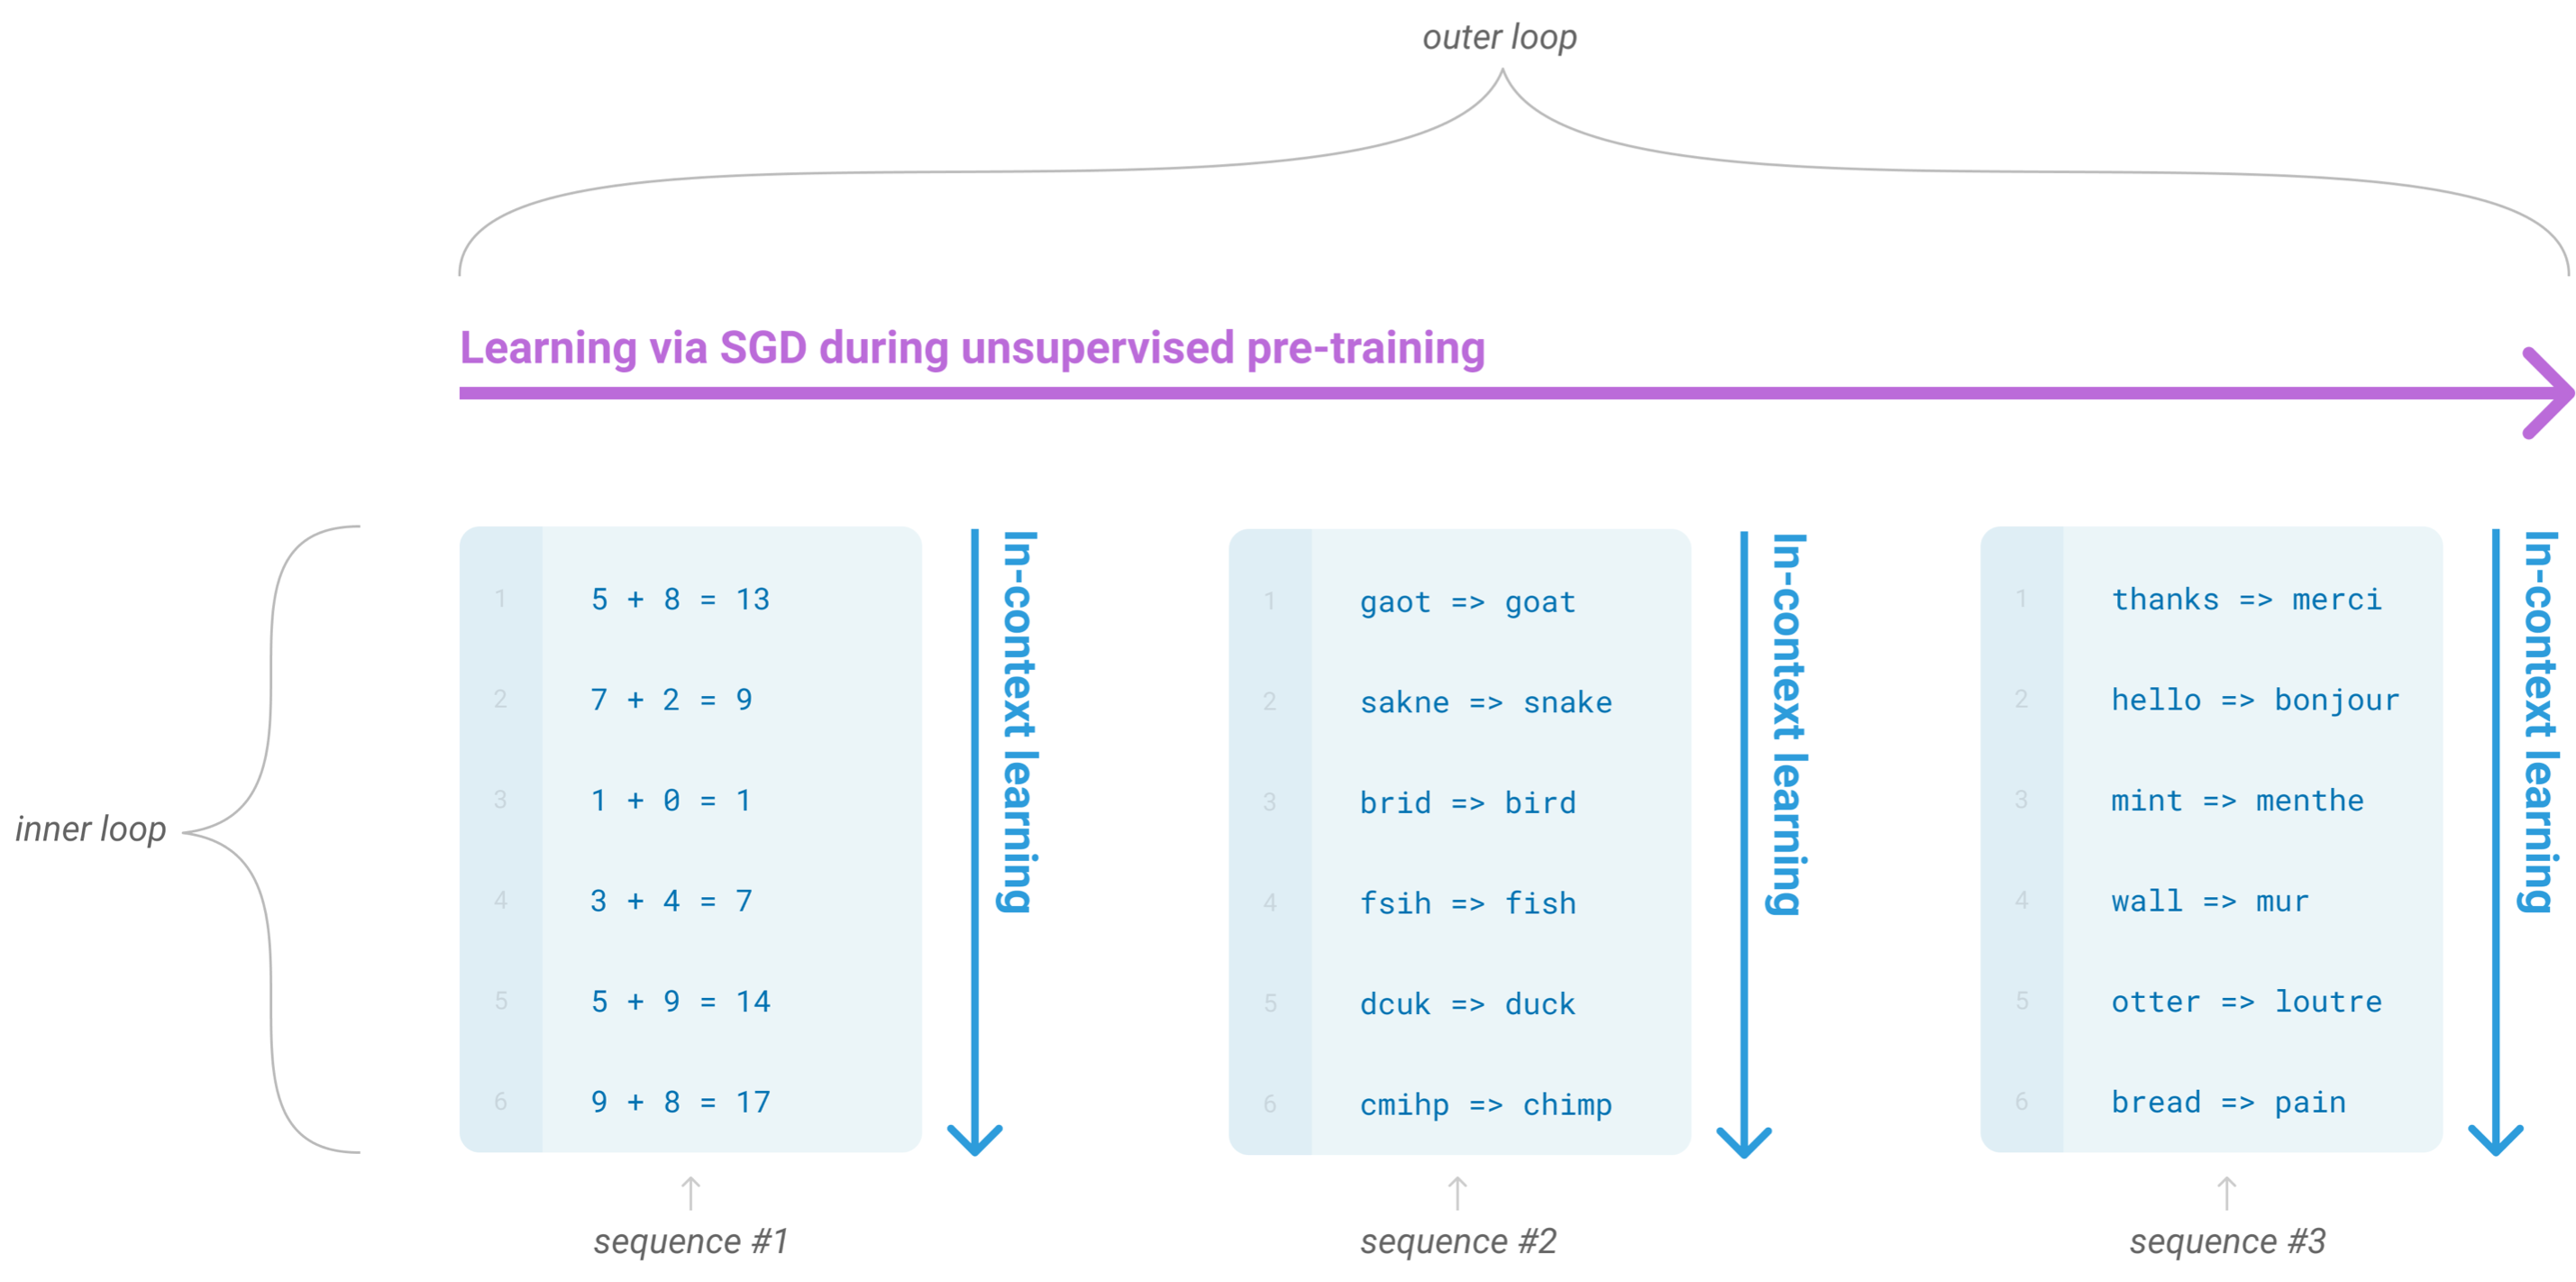
\includegraphics[width=.4\textwidth]{figure/twotypesoflearning.png}\\
\citebutton{Source: Brown et al., 2020}{https://arxiv.org/abs/2005.14165}
\end{figure}
\begin{itemize}
  \item \textbf{Outer loop (pretraining):} the model develops a broad set of skills and abilities, via ordinary gradient descent.
  \item \textbf{Inner loop (inference):} the model uses these abilities to rapidly adapt to a desired task from context alone -- this \textit{is} in-context learning -- in a single forward pass, with no gradient updates at all.
\end{itemize}
\end{vbframe}

\begin{vbframe}{Zero-, One-, and Few-Shot, Side by Side}
\begin{columns}
\column{0.33\textwidth}
\centering
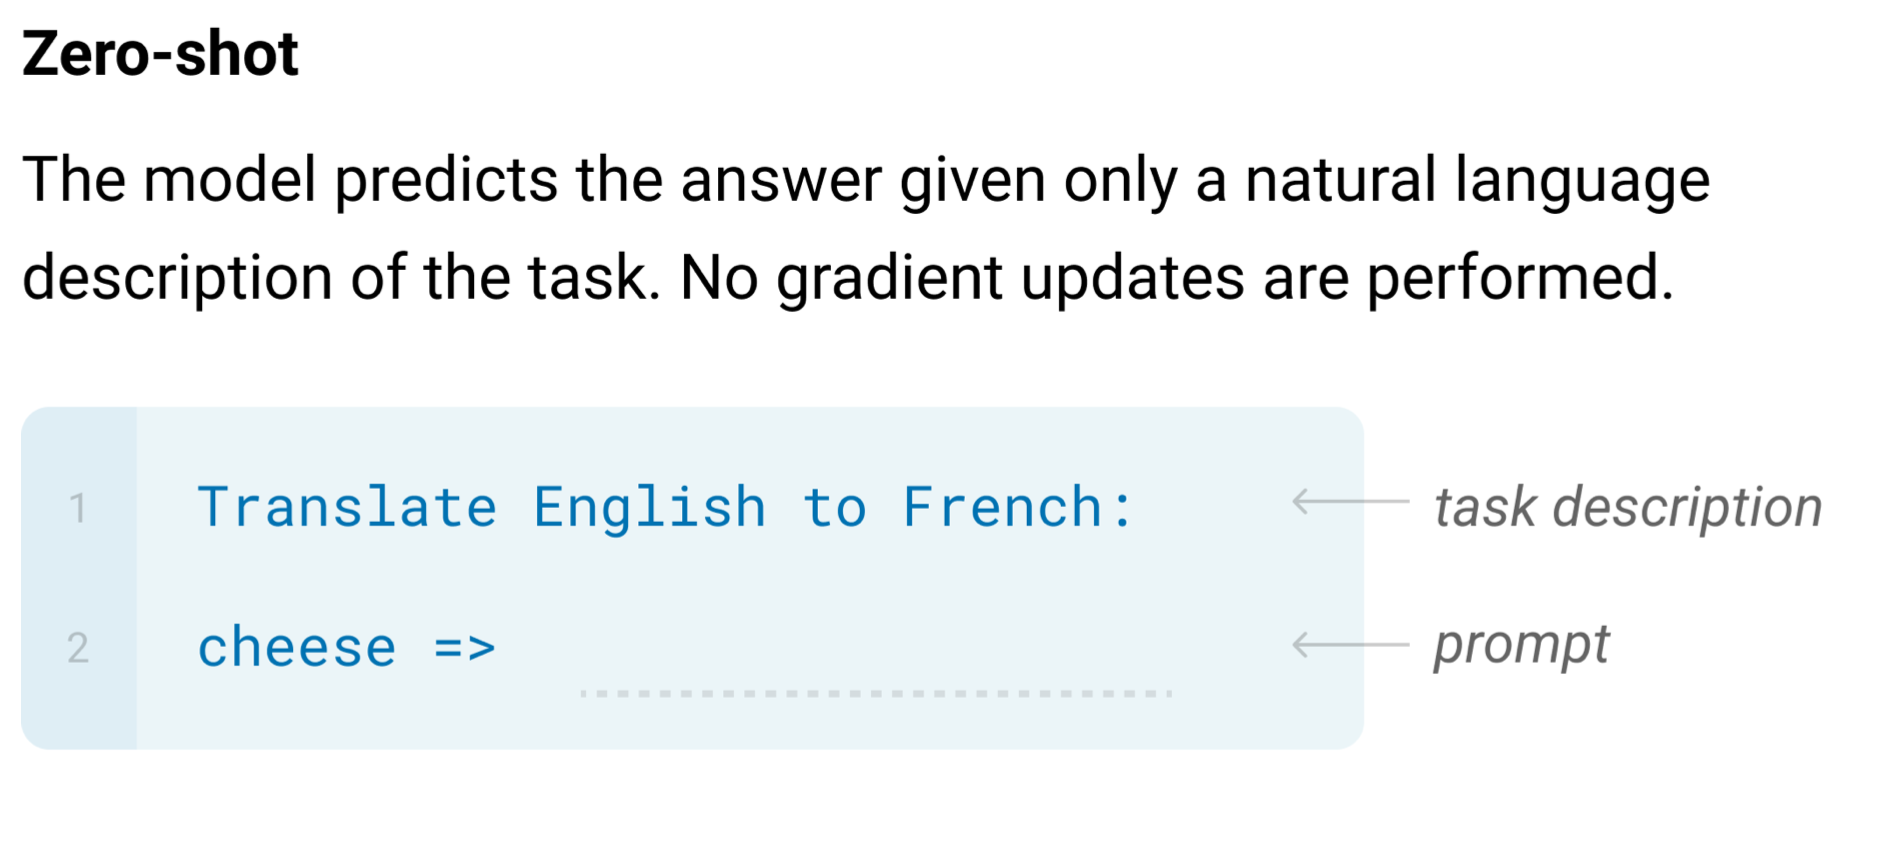
\includegraphics[width=\textwidth]{figure/gptzeroshot.png}\\
\scriptsize zero-shot
\column{0.33\textwidth}
\centering
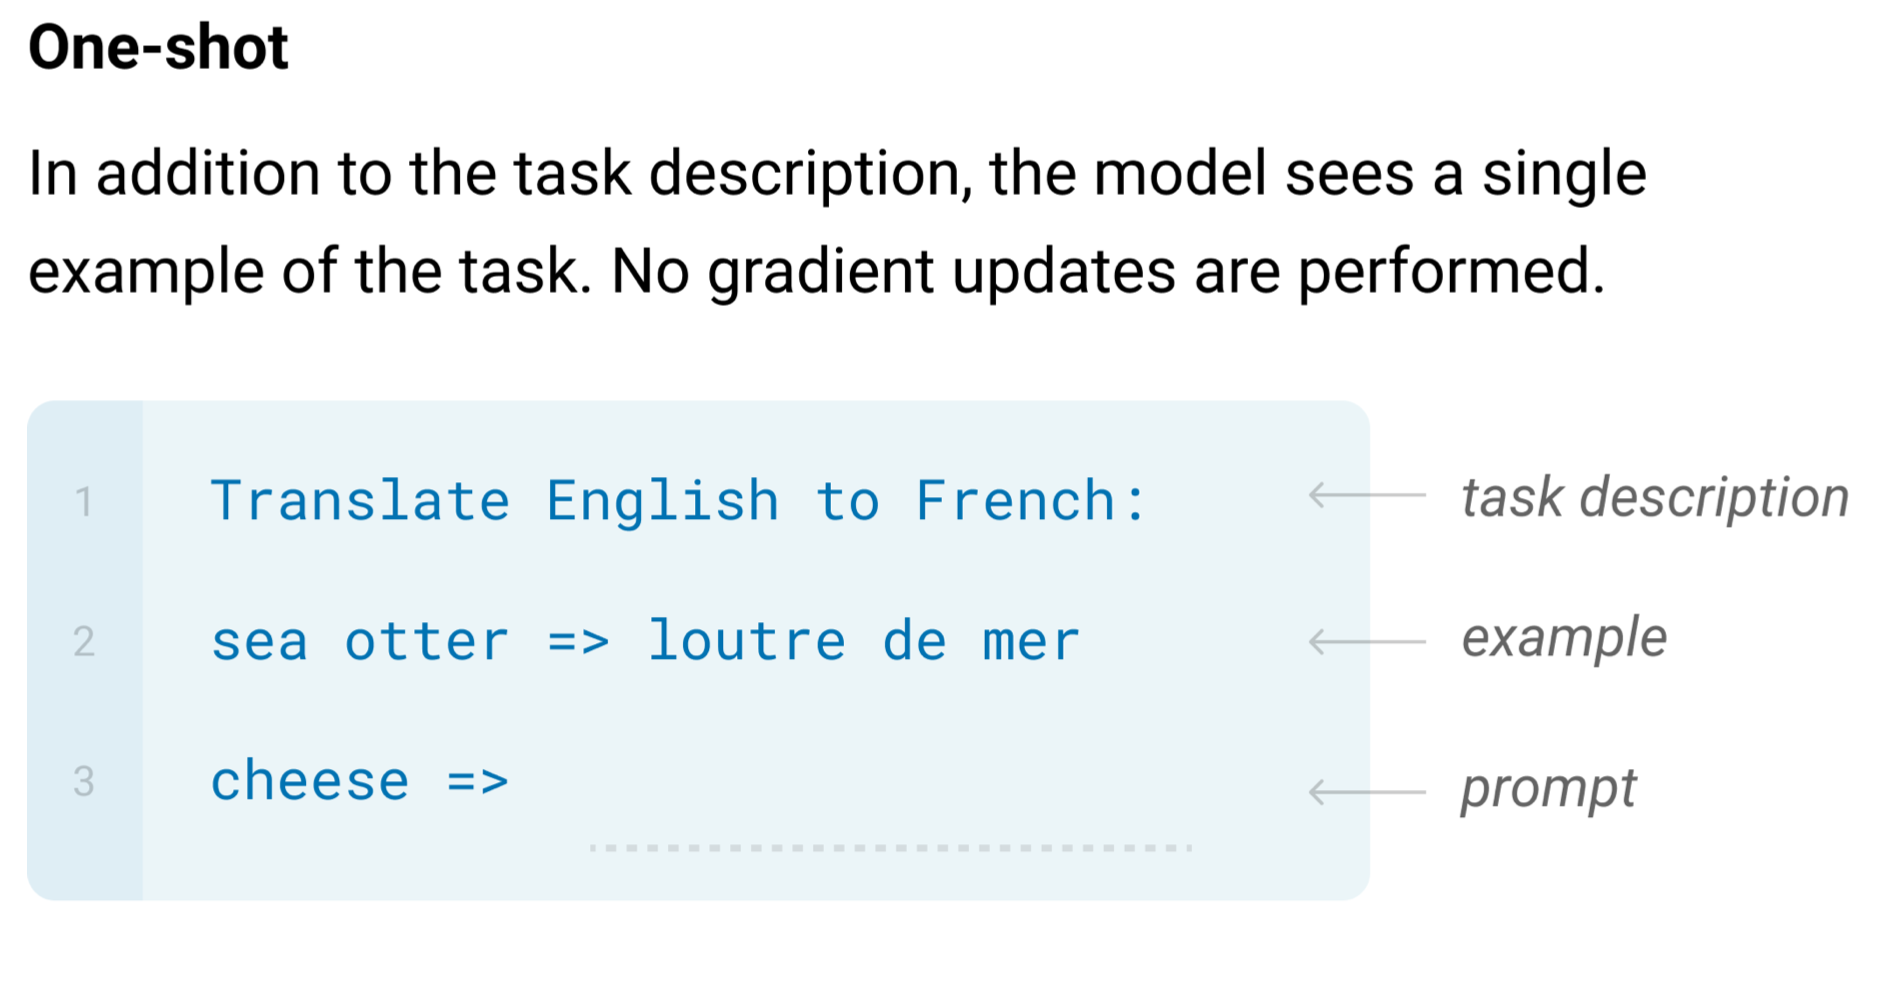
\includegraphics[width=\textwidth]{figure/gptoneshot.png}\\
\scriptsize one-shot
\column{0.33\textwidth}
\centering
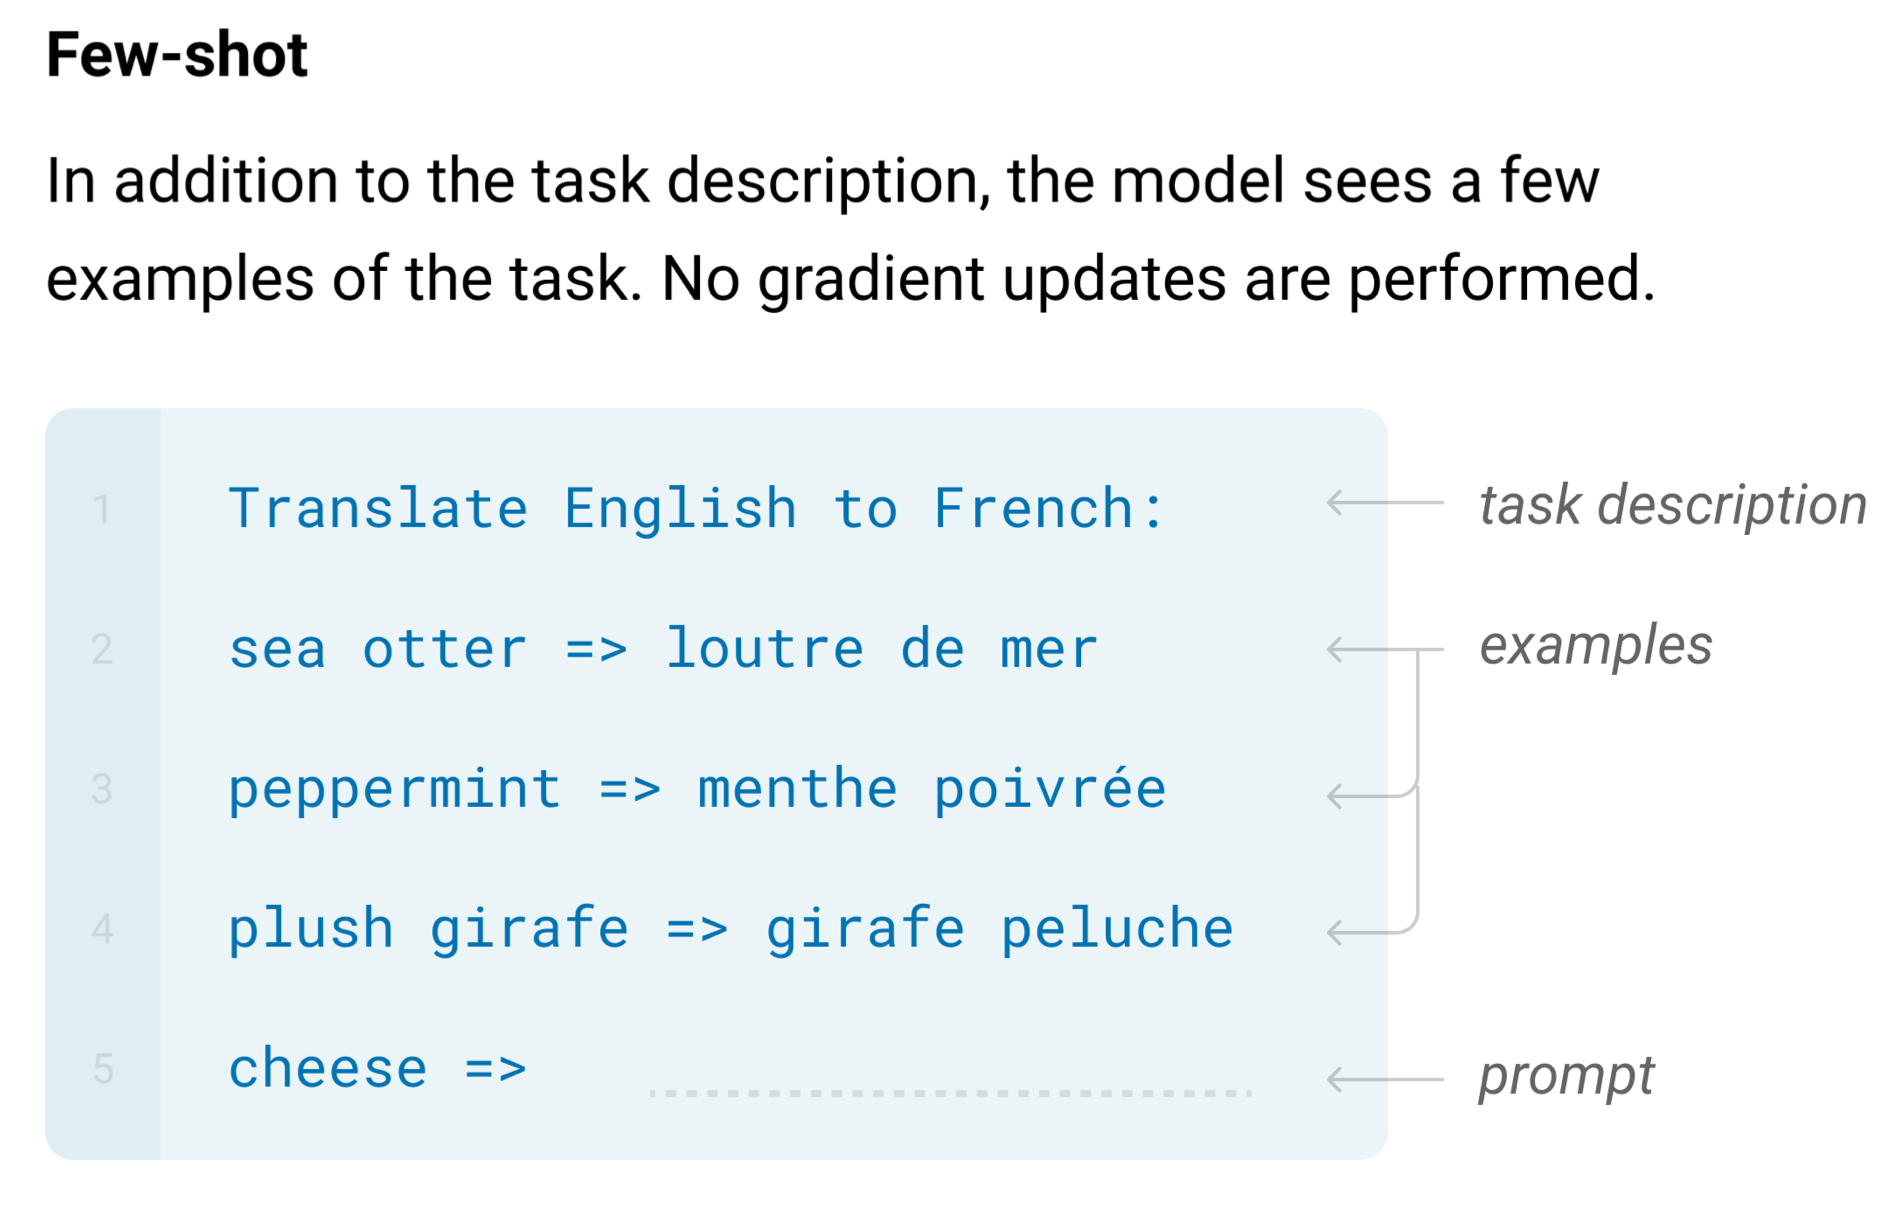
\includegraphics[width=\textwidth]{figure/gptfewshot.png}\\
\scriptsize few-shot
\end{columns}
\vspace{2mm}
\citebutton{Source: Brown et al., 2020}{https://arxiv.org/abs/2005.14165}
\begin{itemize}
  \item In every case: no gradient updates -- the model has to ``understand'' the task description, with progressively more demonstration examples helping it do so.
  \item The number of demonstrations is itself a hyperparameter; larger models make better use of more demonstrations -- few-shot performance scales up faster than zero-shot as model size grows.
\end{itemize}
\end{vbframe}

\begin{vbframe}{GPT-3: Architecture and Training Corpus}
\begin{figure}
\centering
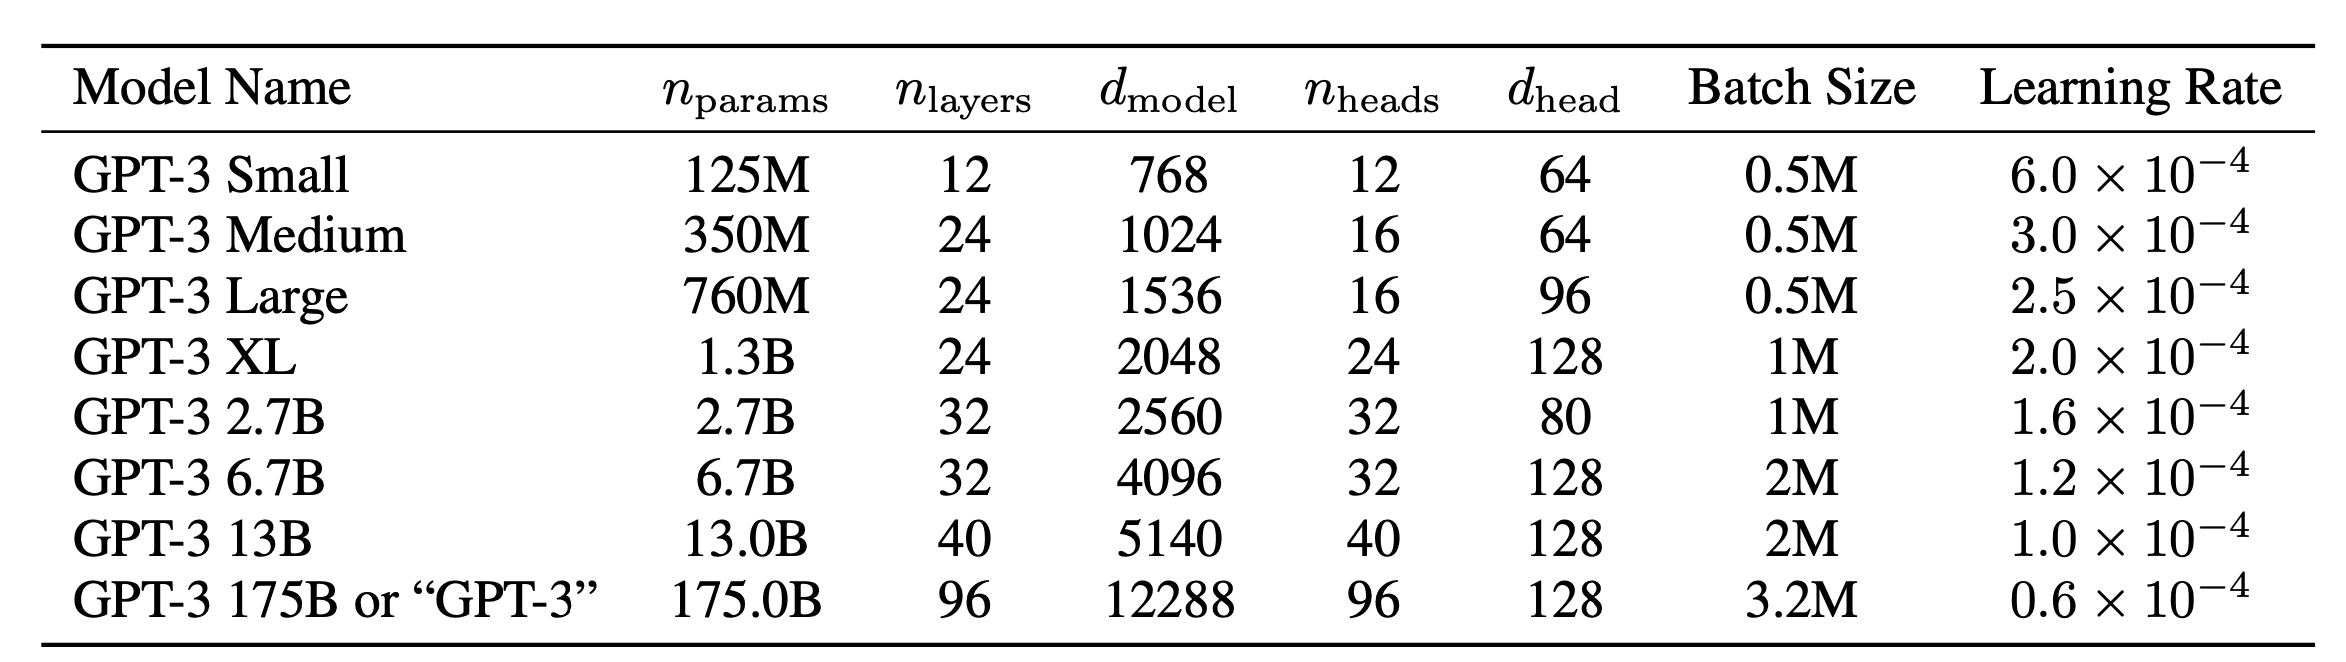
\includegraphics[width=.8\textwidth]{figure/gptarch.png}\\
\citebutton{Source: Brown et al., 2020}{https://arxiv.org/abs/2005.14165}
\end{figure}
\begin{itemize}
  \item ``GPT-3'' usually refers to the largest of several released sizes -- both width ($d_{model}$) and depth ($n_{layers}$) are scaled together, with head count adjusted to $d_{model}$.
  \item Training corpus: BERT used $\sim$3.3B words ($\sim$4--6B tokens); GPT-3 used \textbf{499B tokens} -- two orders of magnitude more, within under two years -- mostly internet text (including, notoriously, some benchmark test sets).
\end{itemize}
\end{vbframe}

\begin{vbframe}{Loss as a Power Law of Compute}
\begin{figure}
\centering
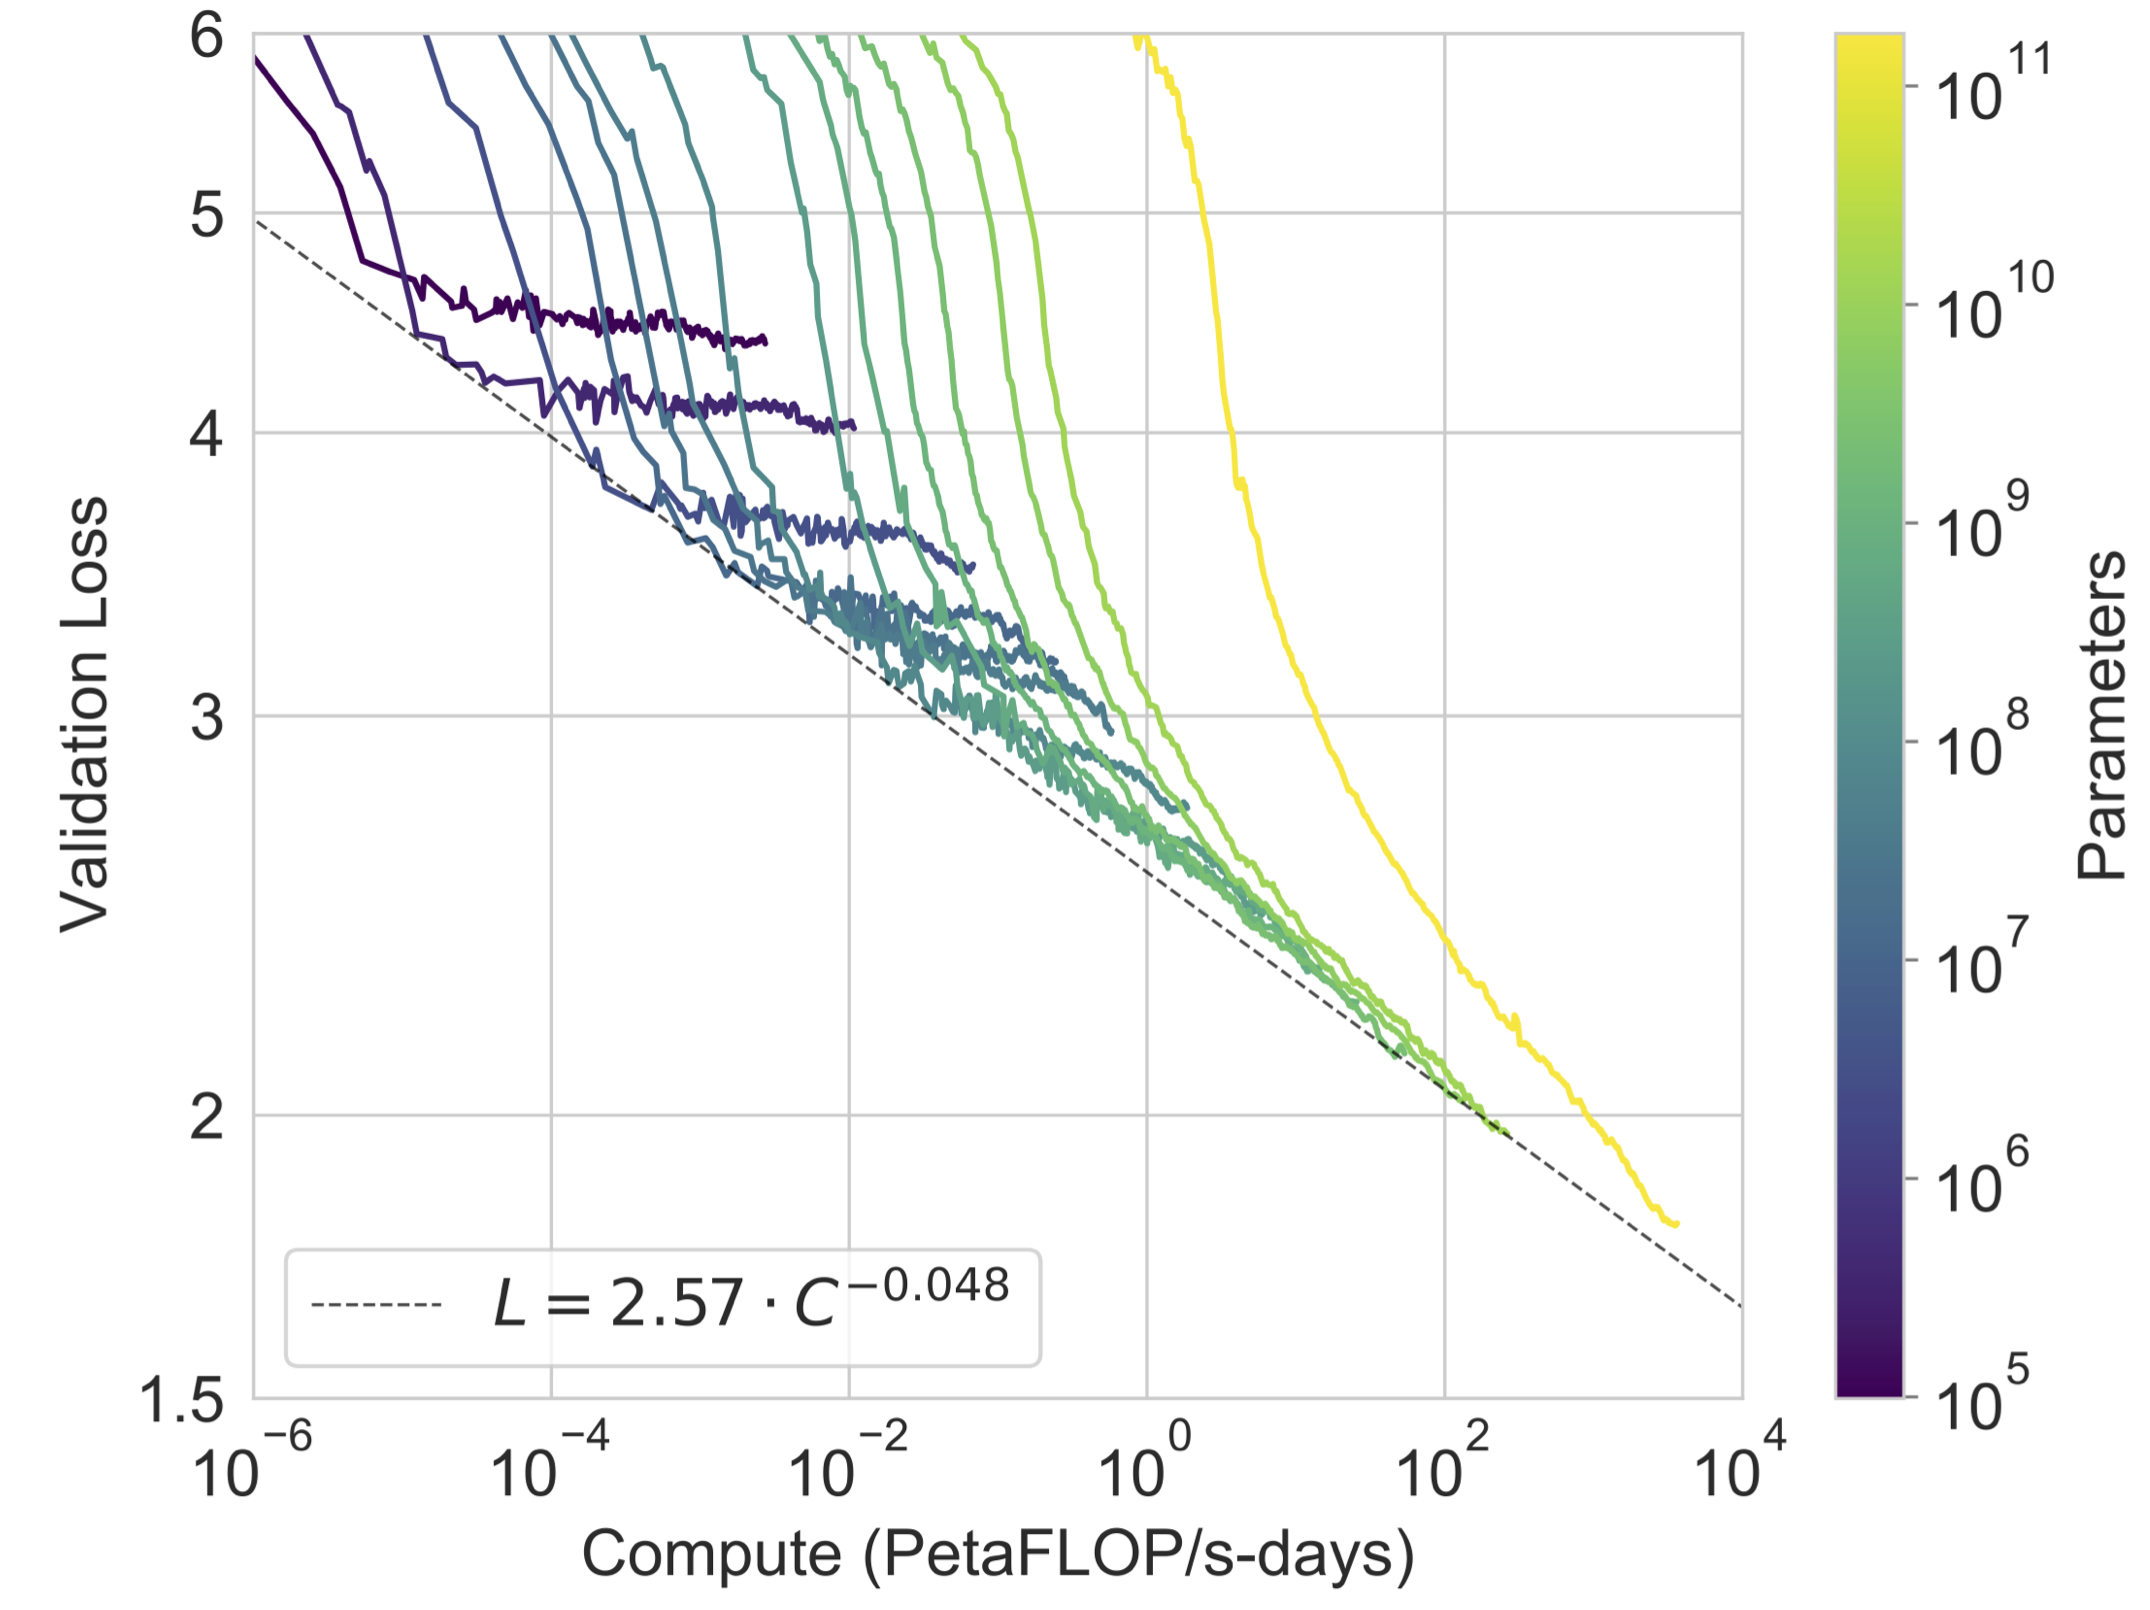
\includegraphics[width=.55\textwidth]{figure/losscompute.png}\\
\citebutton{Source: Brown et al., 2020}{https://arxiv.org/abs/2005.14165}
\end{figure}
\begin{itemize}
  \item Test loss falls smoothly as a \textbf{power law} in training compute, across many orders of magnitude -- this single curve is the empirical seed of the entire scaling-laws literature this session returns to later.
\end{itemize}
\end{vbframe}

%%%%%%%%%%%%%%%%%%%%%%%%%%%%%%%%%%%%%%%%%%%%%%%%%%%%%%%%%%%%%%%%%%

\section{GPT-3: Discussion and Limitations}
%%%%%%%%%%%%%%%%%%%%%%%%%%%%%%%%%%%%%%%%%%%%%%%%%%%%%%%%%%%%%%%%%%

\begin{vbframe}{Can GPT-3 Fool Humans?}
\begin{figure}
\centering
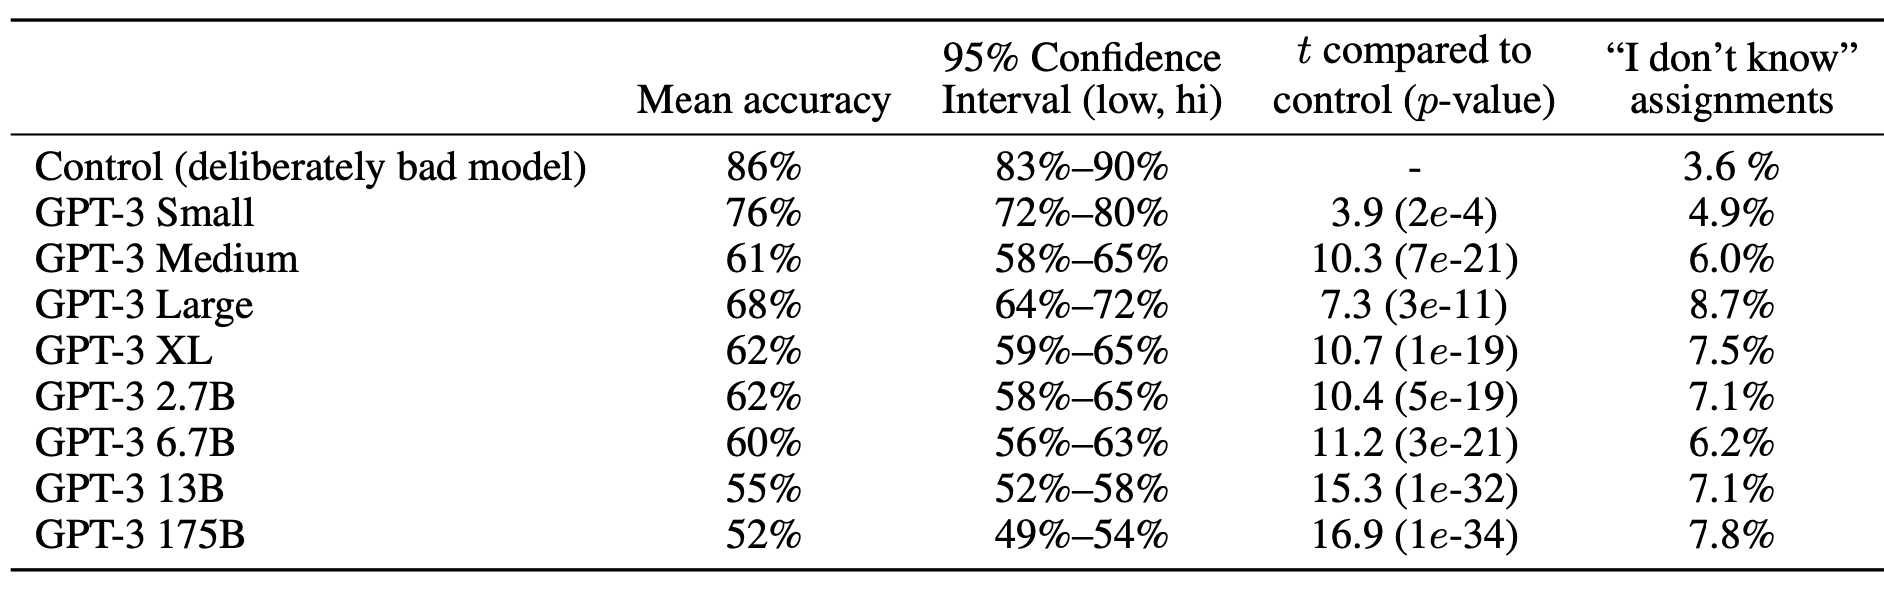
\includegraphics[width=.55\textwidth]{figure/humanvsmachine.png}\\
\citebutton{Source: Brown et al., 2020}{https://arxiv.org/abs/2005.14165}
\end{figure}
\begin{itemize}
  \item Brown et al.\ tested whether human evaluators could distinguish GPT-3-generated news articles from human-written ones -- accuracy for the largest model was close to chance, a Turing-test-style result that drove much of GPT-3's public attention.
\end{itemize}
\end{vbframe}

\begin{vbframe}{Bias}
\begin{figure}
\centering
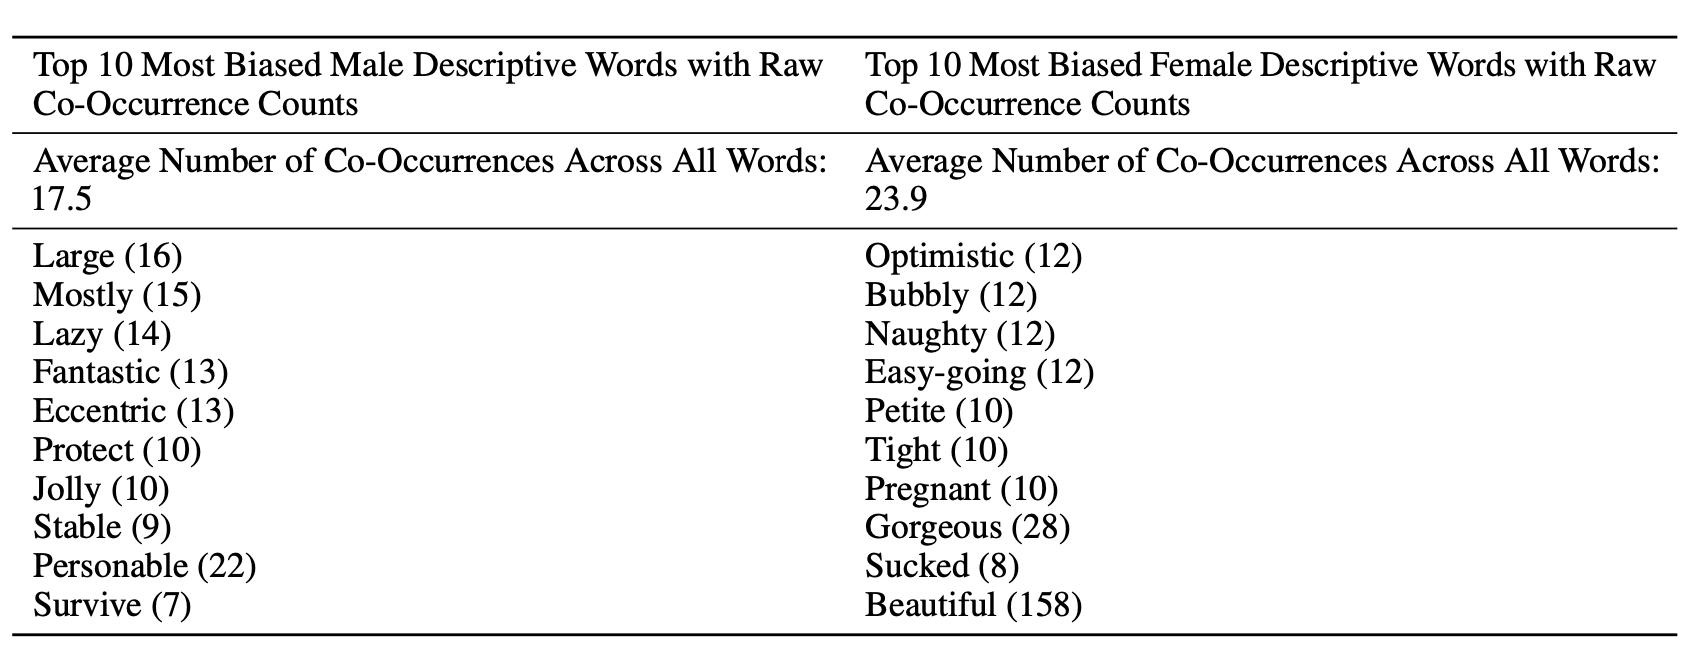
\includegraphics[width=.55\textwidth]{figure/genderbias.png}\\
\citebutton{Source: Brown et al., 2020}{https://arxiv.org/abs/2005.14165}
\end{figure}
\begin{itemize}
  \item Trained on internet-scale text, GPT-3 reproduces the biases present in that text -- gender, race, and religion associations show up systematically in generated completions.
  \item Same underlying issue as BERTology's bias findings in session 8 (StereoSet) -- scale amplifies capability \textit{and} amplifies whatever the training distribution contains.
\end{itemize}
\end{vbframe}

\begin{vbframe}{From GPT-3 to Today}
\begin{itemize}
  \item GPT-3 built directly on GPT-2's foundation: multi-task learning (GPT-2) extended into prompting and in-context learning (GPT-3) -- and then ChatGPT happened.
  \item Models over $200\times$ the size of GPT-2 have since been trained; the Transformer decoder remains the backbone of nearly all of them.
  \item The rest of this session is about everything built \textit{on top} of this decoder-only recipe: how to make it solve tasks reliably (fine-tuning and prompting), how to make it reason (chain-of-thought), what it costs to train, and how far scaling alone can go.
\end{itemize}
\end{vbframe}

%%%%%%%%%%%%%%%%%%%%%%%%%%%%%%%%%%%%%%%%%%%%%%%%%%%%%%%%%%%%%%%%%%

\section{Fine-Tuning and Prompting, Precisely}
%%%%%%%%%%%%%%%%%%%%%%%%%%%%%%%%%%%%%%%%%%%%%%%%%%%%%%%%%%%%%%%%%%

\begin{vbframe}{Why the LM Objective Alone Isn't Enough}
\begin{itemize}
  \item Both masking (BERT) and next-token prediction (GPT) are self-supervised objectives with no explicit notion of ``task'' -- the model learns to predict tokens, not to solve problems.
  \item So turning a pretrained LM into something that reliably solves a specific task requires additional work. GPT-1/2/3 already showed several answers to ``how''; this section makes each one precise.
\end{itemize}
\end{vbframe}

\begin{vbframe}{Single-Task Fine-Tuning, and Verbalizers}
\begin{itemize}
  \item \textbf{``Old-style'' single-task fine-tuning:} supervised training of the pretrained model on a task-specific set of size $k$ (not small, e.g.\ $k=100$). This is the typical way encoder models like BERT are used (session 8), and is still relevant whenever you need a small, efficient, single-purpose model.
  \item The output head can predict an arbitrary category (``0''/``1'' for sentiment) -- or a meaningful \textbf{verbalizer} (``negative''/``positive'') \citebutton{Schick et al., 2020}{https://arxiv.org/abs/2009.07118}.
  \item Verbalizers need \textit{less} data: the pretrained LM already ``understands'' words like ``good''/``bad'' from pretraining, so fine-tuning only has to teach it \textit{when} to use them, not what they mean.
\end{itemize}
\end{vbframe}

\begin{vbframe}{Prompting: Precise Definitions}
\begin{itemize}
  \item Prompting always means \myblue{no fine-tuning} -- the model's parameters never change.
  \item Originally: carefully \myblue{designing the input} to elicit a desired output. Today, any input to the model is loosely called a ``prompt''.
  \item \myblue{Few-shot ($k$-shot) prompting}: give $k$ examples of the desired behavior as part of the input.
  \item \myblue{Zero-shot prompting}: give no examples ($k=0$) -- the term is used precisely to contrast with $k>0$.
  \item Prompting = instruction = task description = pattern -- several names for the same idea, all seen already in GPT-2's and GPT-3's zero/few-shot frames above.
\end{itemize}
\end{vbframe}

\begin{vbframe}{Multi-Task Fine-Tuning: T0, T5, FLAN}
\begin{itemize}
  \item \textbf{Multi-task fine-tuning:} fine-tune on a large training set spanning \textit{many} tasks -- generally, the more tasks the better.
  \item Two flavors: a \textbf{consistent} task format (every task reformulated the same way, e.g.\ T5's text-to-text prefixes, session 8) vs.\ a more \textbf{open} format with per-task instructions.
  \item T5's approach is \textit{non-unified}: the model implicitly learns, via fine-tuning, which prefix maps to which label set -- raising a genuine question of how well this generalizes to a truly new, unseen task. \citebutton{Source: Wei et al., 2021}{https://arxiv.org/abs/2109.01652}
\end{itemize}
\end{vbframe}

\begin{vbframe}{Multitask Prompted Training: Held-Out \textit{Tasks}}
\begin{itemize}
  \item T0 \citebutton{Sanh et al., 2021}{https://arxiv.org/abs/2110.08207} makes the format \textit{unified}: many tasks share a common prompt template, explicitly aiming to generalize to genuinely new tasks.
  \item Evaluation changes accordingly: instead of held-out \textit{samples} (standard in NLP), T0 uses held-out \textit{tasks} -- every dataset belonging to a held-out task goes entirely into the test set. This directly tests generalization across tasks, not just across examples of the same task.
\end{itemize}
\end{vbframe}

\begin{vbframe}{Instruction Tuning: Terminology}
\begin{itemize}
  \item The term ``instruction tuning'' was introduced by the FLAN paper \citebutton{Source: Wei et al., 2021}{https://arxiv.org/abs/2109.01652} -- but today it covers something broader than multi-task fine-tuning on classical NLP tasks.
  \item Modern instruction tuning also covers open-ended generation and ``alignment'': brainstorming, writing a joke, giving analogies, refusing hateful requests -- none of these are classical NLP tasks.
  \item \textbf{This course's terminology:} \textit{multi-task fine-tuning} = tasks in the classical NLP sense; \textit{instruction tuning} = the broader project of shaping a raw next-token predictor into something ``helpful, harmless, and honest'' -- of which classical-task fine-tuning is just one part.
  \item Instruction tuning and reinforcement learning from human feedback (RLHF) are both, in this broader sense, forms of fine-tuning -- RLHF is session 11's subject.
\end{itemize}
\end{vbframe}

\begin{vbframe}{Fine-Tuning: Conclusions}
\begin{itemize}
  \item More training tasks $\to$ better generalization, and multi-task fine-tuning transfers across architectures.
  \item It greatly improves usability, and it is \textit{cheap} relative to pretraining: for PaLM 540B, instruction tuning took only 0.2\% of pretraining compute, yet improved performance by 9.4\% -- a striking cost/benefit ratio that partly explains why fine-tuning/prompting research exploded once large pretrained models existed.
\end{itemize}
\end{vbframe}

%%%%%%%%%%%%%%%%%%%%%%%%%%%%%%%%%%%%%%%%%%%%%%%%%%%%%%%%%%%%%%%%%%

\section{Chain-of-Thought Reasoning}
%%%%%%%%%%%%%%%%%%%%%%%%%%%%%%%%%%%%%%%%%%%%%%%%%%%%%%%%%%%%%%%%%%

\begin{vbframe}{The Problem: LLMs Are Bad at Multi-Step Reasoning}
\begin{itemize}
  \item Even very large LMs struggle with tasks that require chaining several intermediate steps -- arithmetic, symbolic manipulation, multi-hop question answering -- when asked to jump straight to the final answer.
  \item \ques How to boost the reasoning capabilities of LMs? \citebutton{Wei et al., 2021}{https://arxiv.org/abs/2109.01652}
\end{itemize}
\end{vbframe}

\begin{vbframe}{Chain-of-Thought Prompting}
\begin{figure}
\centering
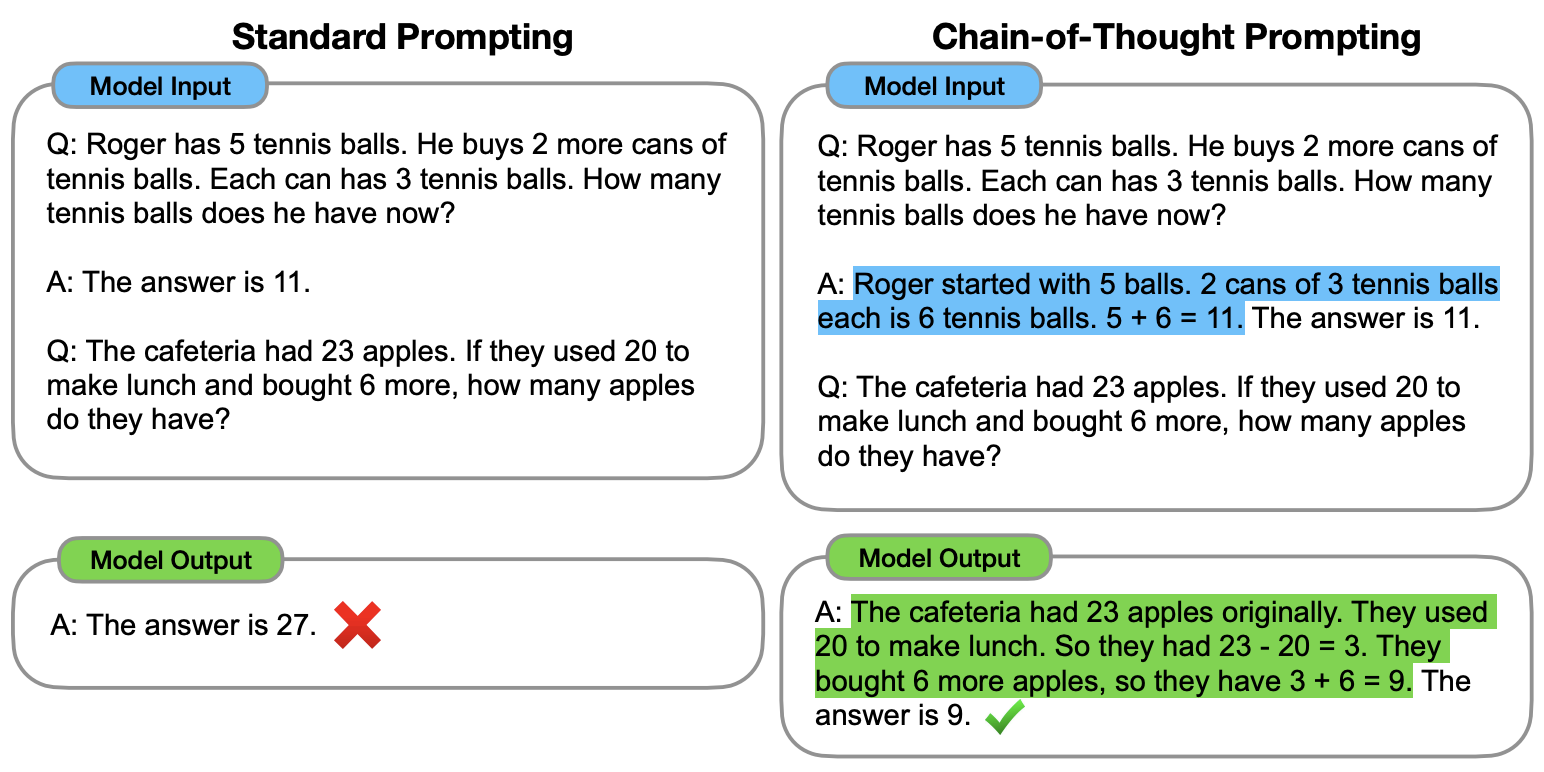
\includegraphics[width=.85\textwidth]{figure/chain_of_thought.png}\\
\citebutton{Source: Wei et al., 2022}{https://arxiv.org/pdf/2201.11903.pdf}
\end{figure}
\begin{itemize}
  \item Standard few-shot prompting shows only (question, final answer) pairs. \textbf{Chain-of-thought (CoT) prompting} shows (question, \textit{reasoning steps}, final answer) instead -- and the model imitates the reasoning steps at inference time, not just the answer format.
\end{itemize}
\end{vbframe}

\begin{vbframe}{A Worked Example}
\begin{figure}
\centering
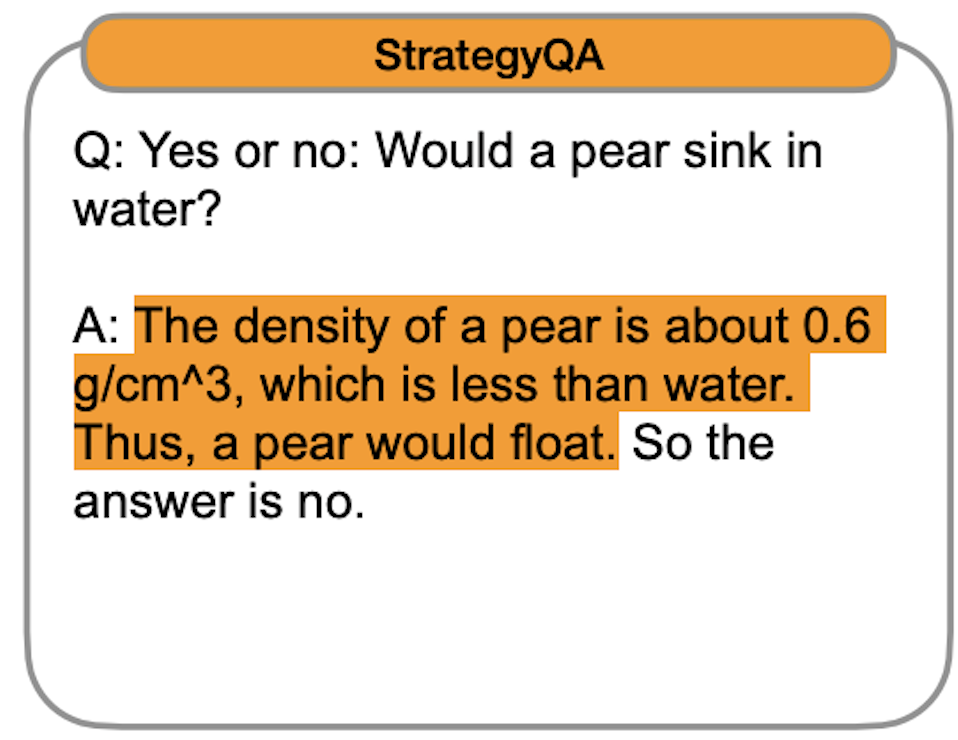
\includegraphics[height=6cm]{figure/cotex1.png}\\
\citebutton{Source: Wei et al., 2022}{https://arxiv.org/pdf/2201.11903.pdf}
\end{figure}
\begin{itemize}
  \item Writing out intermediate arithmetic explicitly, rather than jumping to the number, is enough to unlock correct answers on problems the same model fails without it.
\end{itemize}
\end{vbframe}

\begin{vbframe}{Chain-of-Thought Only Helps Large Models}
\begin{figure}
\centering
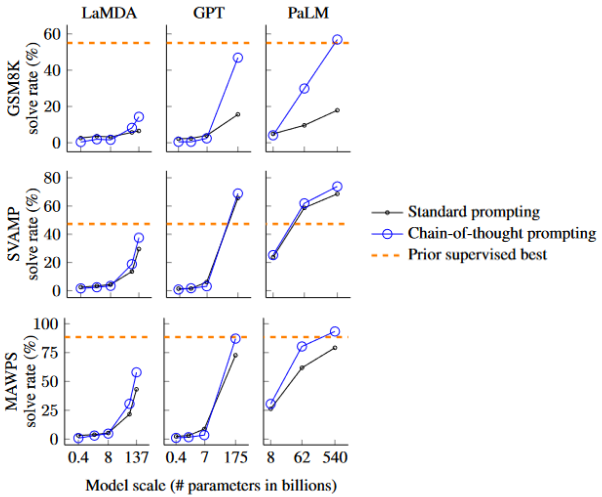
\includegraphics[width=.65\textwidth]{figure/cot_performance1.png}\\
\citebutton{Source: Wei et al., 2022}{https://arxiv.org/pdf/2201.11903.pdf}
\end{figure}
\begin{itemize}
  \item CoT prompting is an \textbf{emergent} benefit: below a certain model scale it doesn't help (or even hurts), and above it, gains grow sharply -- another data point for ``scale changes what a model can do,'' revisited critically two sections from now.
\end{itemize}
\end{vbframe}

\begin{vbframe}{Tree-of-Thought: Beyond a Single Chain}
\begin{figure}
\centering
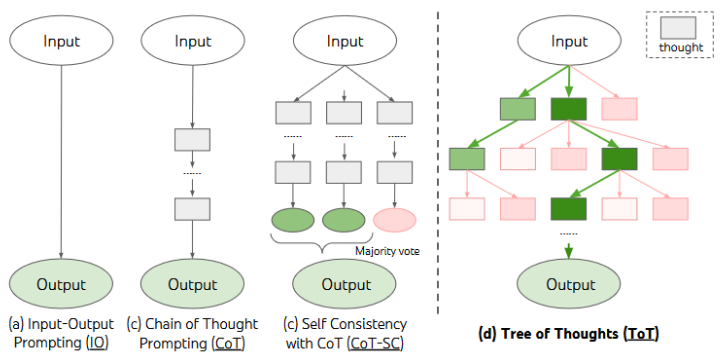
\includegraphics[width=.7\textwidth]{figure/tot_vs_cot.png}\\
\citebutton{Yao et al., 2023}{https://arxiv.org/pdf/2305.10601.pdf}
\end{figure}
\begin{itemize}
  \item CoT commits to a single linear reasoning path. \textbf{Tree-of-thought} instead explores multiple candidate reasoning steps at each point, evaluates them, and can backtrack -- deliberate search over reasoning paths rather than one greedy chain. This idea reappears, in a very different (RL-trained) form, in DeepSeek-R1 later.
\end{itemize}
\end{vbframe}

\begin{vbframe}{A Caveat: Is the Chain of Thought \textit{Faithful}?}
\begin{itemize}
  \item CoT reasoning traces \textit{look} like the model's actual computation -- but a written explanation is not guaranteed to be the true causal process behind the answer.
  \item Keep this question open: this session's DeepSeek section returns to it with a concrete example of a model reasoning traces that don't match how the answer was actually produced.
\end{itemize}
\end{vbframe}

%%%%%%%%%%%%%%%%%%%%%%%%%%%%%%%%%%%%%%%%%%%%%%%%%%%%%%%%%%%%%%%%%%

\section{Emergent Abilities: A Real Effect, or a Mirage?}
%%%%%%%%%%%%%%%%%%%%%%%%%%%%%%%%%%%%%%%%%%%%%%%%%%%%%%%%%%%%%%%%%%

\begin{vbframe}{Emergent Abilities: The Claim}
\begin{itemize}
  \item \textbf{Claim:} as model scale increases, some abilities appear discontinuously -- near-random performance below a threshold scale, then a sharp jump above it -- rather than improving smoothly. \citebutton{Wei et al., 2022}{https://arxiv.org/abs/2206.07682}
  \item Chain-of-thought's own scale-dependence, on the previous slide, is one commonly-cited example.
  \item If real, this is important and slightly alarming: it means new capabilities (good \textit{or} bad) could appear at some future scale without a way to predict them from smaller models' behavior in advance.
\end{itemize}
\end{vbframe}

\begin{vbframe}{The Skeptical Counter-View}
\begin{itemize}
  \item Schaeffer et al.\ (2023) argue emergence is often a \textbf{mirage of metric choice}, not of the underlying model: \citebutton{Source: Schaeffer et al., 2023}{https://arxiv.org/pdf/2304.15004.pdf}
  \item Many ``emergent'' results use a discontinuous metric (e.g.\ exact-match accuracy on multi-token answers). Switch to a continuous, token-level metric on the \textit{same} model outputs, and the same results often become smooth, predictable curves.
  \item Lesson for this course's persona: a striking empirical claim about scale is exactly the kind of result to be suspicious of before believing -- check whether the effect survives a change of metric, not just a change of model.
\end{itemize}
\end{vbframe}

%%%%%%%%%%%%%%%%%%%%%%%%%%%%%%%%%%%%%%%%%%%%%%%%%%%%%%%%%%%%%%%%%%

\section{Training LLMs: Compute}
%%%%%%%%%%%%%%%%%%%%%%%%%%%%%%%%%%%%%%%%%%%%%%%%%%%%%%%%%%%%%%%%%%

\begin{vbframe}{The Compute Equation}
$$C \approx \tau T = 6PD$$
\begin{itemize}
  \item $\tau$: hardware throughput (\#GPUs $\times$ FLOPs/GPU); $T$: training time in seconds; $P$: number of parameters; $D$: dataset size, in tokens.
  \item $C = C_{forward} + C_{backward}$, with $C_{forward}\approx 2PD$ and $C_{backward}\approx 4PD$: the factor 2 comes from the multiply-accumulate in matrix multiplication, and the backward pass costs roughly twice the forward pass, since gradients must be computed both for each layer's weights and for the previous layer's outputs.
  \item Measured in FLOP-seconds (also GFLOP-/TFLOP-/PFLOP-days) or GPU-hours; actual achieved FLOPs are always below the advertised theoretical peak.
  \item \citebutton{Source: Quentin et al., 2023}{https://blog.eleuther.ai/transformer-math/}
\end{itemize}
\end{vbframe}

\begin{vbframe}{Parameters vs.\ Dataset: A First Look at the Tradeoff}
\begin{itemize}
  \item Performance depends on \textit{both} $P$ and $D$, not just model size -- so for a fixed compute budget $C=6PD$, there is a tradeoff between training a bigger model on less data or a smaller model on more.
  \item One proposed rule of thumb, $D=20P$, was posited for the Chinchilla models \citebutton{Hoffmann et al., 2022}{https://arxiv.org/abs/2203.15556} -- no longer seen as universally valid (see the scaling-laws section below).
  \item In practice, model size is chosen either from an available compute budget, or from a target inference-time performance (e.g.\ tokens/second) -- two different optimization problems with different answers.
\end{itemize}
\end{vbframe}

\begin{vbframe}{Compute is Only Half the Story}
\begin{itemize}
  \item Even with unlimited FLOPs, a model has to physically \textit{fit} in GPU memory to train at all. Two recurring practical questions: how big is this model in bytes, and will it fit/train on my GPUs?
  \item Four contributors to training memory: model \textbf{parameters}, \textbf{optimizer states}, \textbf{gradients}, and \textbf{activations} -- each explored next.
\end{itemize}
\end{vbframe}

%%%%%%%%%%%%%%%%%%%%%%%%%%%%%%%%%%%%%%%%%%%%%%%%%%%%%%%%%%%%%%%%%%

\section{Training LLMs: Memory}
%%%%%%%%%%%%%%%%%%%%%%%%%%%%%%%%%%%%%%%%%%%%%%%%%%%%%%%%%%%%%%%%%%

\begin{vbframe}{Number Representations}
\begin{figure}
\centering
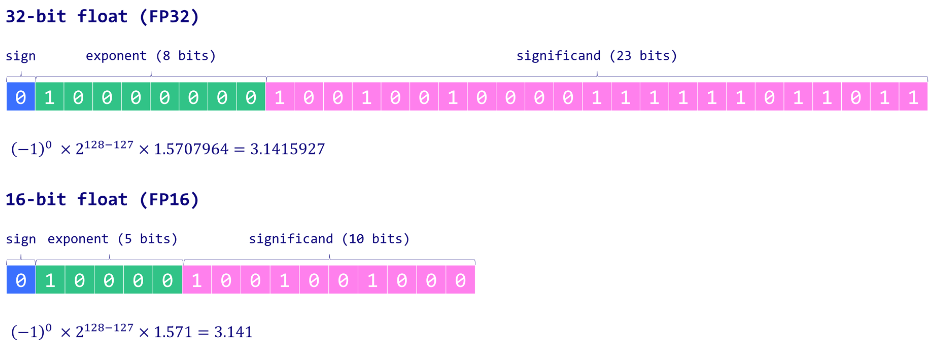
\includegraphics[width=.85\textwidth]{figure/float.png}
\end{figure}
\begin{itemize}
  \item Every float can be written as $(-1)^S\cdot 2^{e-bias}\cdot 1.m$.
  \item \textbf{fp32:} IEEE 754 single precision, 32 bits (4 bytes). \textbf{fp16:} IEEE 754-2008 half precision, 16 bits (2 bytes). \textbf{bf16} (Google Brain): also 16 bits, but fewer significand bits than fp16 (less precise) and more exponent bits (larger dynamic range, so less prone to over/underflow). \textbf{INT8:} 8 bits (1 byte), integer.
  \item \citebutton{(Maxime Labonne)}{https://mlabonne.github.io/blog/posts/Introduction_to_Weight_Quantization.html}
\end{itemize}
\end{vbframe}

\begin{vbframe}{Quantization, at a Glance}
\begin{itemize}
  \item Fitting meaningful values into 8 bits is harder than it sounds -- one alternative is to store an integer plus a scaling factor: $\text{real} = \text{stored\_int}\times\text{scale}$.
  \item \textbf{Absmax (symmetric):} scale by the maximum absolute value in the tensor.
  \item \textbf{Zero-point (asymmetric):} scale and shift so the tensor's actual min/max map onto the full INT8 range -- makes better use of the available integers when values aren't centered at zero.
  \item Active area of research: newer formats like NVFP4 push this even further \citebutton{Link: Nvidia paper on NVFP4}{https://arxiv.org/pdf/2509.25149}.
\end{itemize}
\end{vbframe}

\begin{vbframe}{Putting It Together: Total Training Memory}
\begin{itemize}
  \item \textbf{Parameters:} 4/2/1 bytes per parameter for fp32/fp16-bf16/INT8.
  \item \textbf{Optimizer states (AdamW):} 8 bytes/param (4 for momentum, 4 for variance) -- often the single largest contributor, larger than the parameters themselves. An 8-bit optimizer (bitsandbytes) cuts this to 2 bytes/param.
  \item \textbf{Gradients:} stored in the same dtype as the parameters, so 4/2/1 bytes/param again.
  \item \textbf{Activations:} GPUs are bottlenecked by memory, not FLOPs -- so it is often worth \textit{recomputing} some activations during the backward pass instead of storing them all.
\end{itemize}
$$Mem_{training} = Mem_{params} + Mem_{opt} + Mem_{grad} \,(+\, Mem_{activ})$$
\end{vbframe}

%%%%%%%%%%%%%%%%%%%%%%%%%%%%%%%%%%%%%%%%%%%%%%%%%%%%%%%%%%%%%%%%%%

\section{Training LLMs: Distributed and Efficient}
%%%%%%%%%%%%%%%%%%%%%%%%%%%%%%%%%%%%%%%%%%%%%%%%%%%%%%%%%%%%%%%%%%

\begin{vbframe}{Data Parallelism}
\begin{figure}
\centering
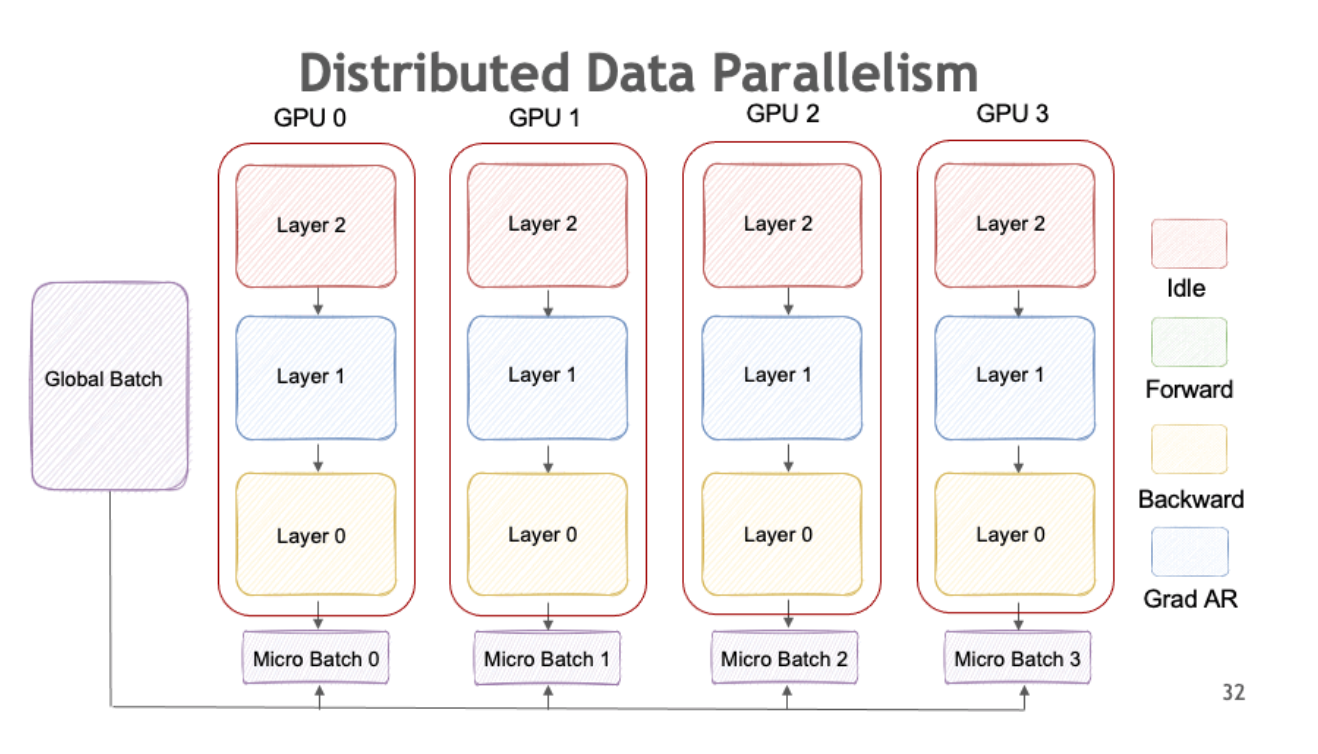
\includegraphics[width=.8\textwidth]{figure/data_parallel.png}\\
{\footnotesize Source: \href{https://docs.nvidia.com/nemo-framework/user-guide/latest/nemotoolkit/features/parallelisms.html#distributed-data-parallelism}{Nvidia}}
\end{figure}
\begin{itemize}
  \item Split the \textit{data} across GPUs, each holding a full model replica. Gradients are computed locally, then averaged across GPUs (all-reduce), and every replica's parameters are updated in sync.
\end{itemize}
\end{vbframe}

\begin{vbframe}{Tensor Parallelism}
\begin{figure}
\centering
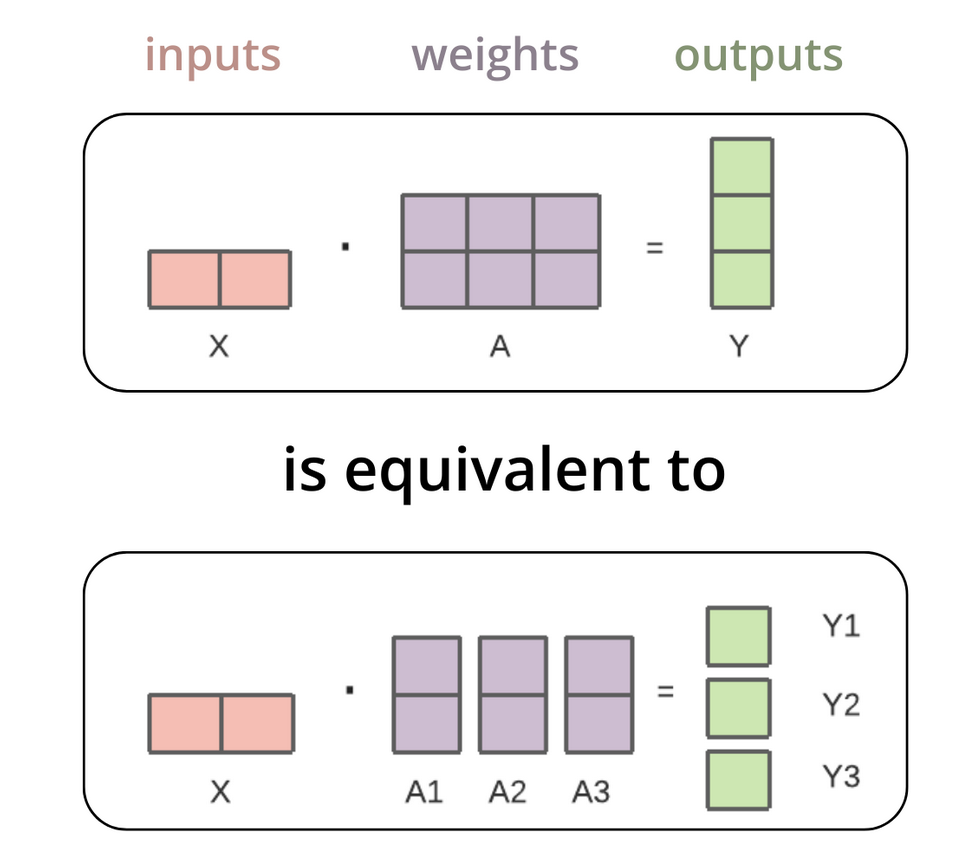
\includegraphics[width=.5\textwidth]{figure/tensor,parallelism,new.png}\\
{\footnotesize Source: \href{https://docs.nvidia.com/nemo-framework/user-guide/latest/nemotoolkit/features/parallelisms.html#tensor-parallelism}{Nvidia}}
\end{figure}
\begin{itemize}
  \item Split the \textit{model's parameters} themselves across GPUs -- necessary once a single model no longer fits on one device, regardless of how the data is split. Forward and backward passes require intermediate results to be exchanged between devices at each split point.
\end{itemize}
\end{vbframe}

\begin{vbframe}{Why Attention Needs Its Own Optimization}
\begin{minipage}[c]{.49\textwidth}
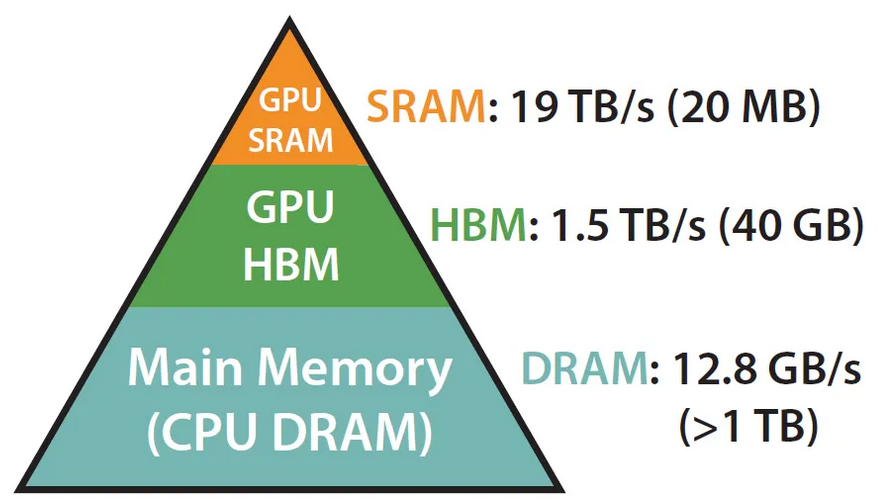
\includegraphics[width=.85\textwidth]{figure/gpu_mem.png}
\end{minipage}
\begin{minipage}[c]{.49\textwidth}
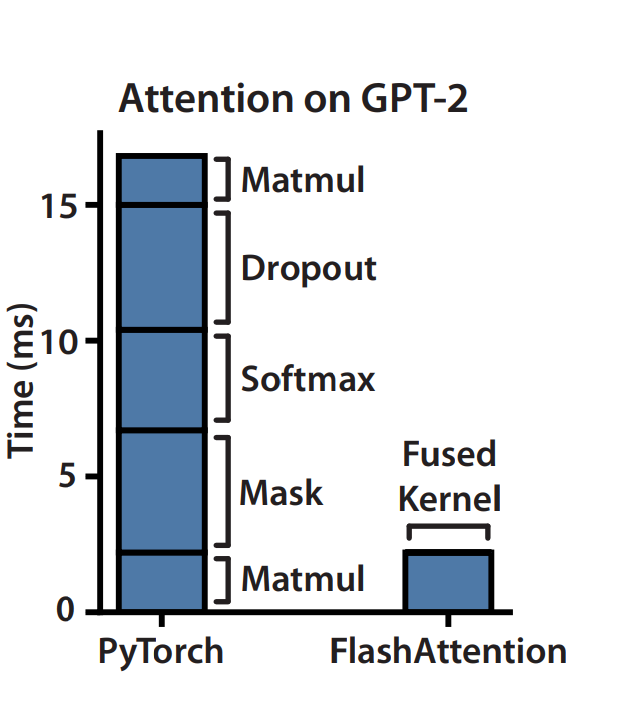
\includegraphics[width=.7\textwidth]{figure/flash-attn.png}
\end{minipage}
\begin{itemize}
  \item GPU compute (FLOPs) is extremely fast; moving data between memory tiers is slow. Attention involves large intermediate $n\times n$ score matrices -- exactly the $O(n^2)$ cost flagged back in session 7 -- so naive attention is \textbf{memory-bound}, not compute-bound: the GPU spends most of its time waiting on data, not computing.
  \item \citebutton{Source: Dao, 2022}{https://arxiv.org/abs/2205.14135}
\end{itemize}
\end{vbframe}

\begin{vbframe}{FlashAttention: Exact, Memory-Efficient, IO-Aware}
\begin{itemize}
  \item \textbf{Memory-efficient:} reduces memory from $O(n^2)$ to $O(n)$ by never materializing the full $n\times n$ score matrix.
  \item \textbf{IO-aware:} uses \textbf{tiling} (chunking $Q$, $K$, $V$ into blocks that fit in fast on-chip SRAM) and \textbf{operation fusion} (query-key matmul, softmax, and value matmul run as one fused kernel) -- this avoids repeatedly writing large intermediate tensors out to slow HBM and reading them back.
  \item \textbf{Exact:} computes the \textit{same} attention as the vanilla formula -- not an approximation, unlike the local/global sparsity tricks from session 7's efficient-attention section. The bigger the attention matrices, the more this helps, until $O(n)$ itself no longer fits.
  \item Limitation: requires a custom CUDA kernel per attention variant, so it doesn't transfer automatically across new attention mechanisms or hardware.
\end{itemize}
\end{vbframe}

%%%%%%%%%%%%%%%%%%%%%%%%%%%%%%%%%%%%%%%%%%%%%%%%%%%%%%%%%%%%%%%%%%

\section{Scaling Laws}
%%%%%%%%%%%%%%%%%%%%%%%%%%%%%%%%%%%%%%%%%%%%%%%%%%%%%%%%%%%%%%%%%%

\begin{vbframe}{Kaplan et al.\ (2020): Power Laws}
\href{https://arxiv.org/abs/2001.08361}{\beamergotobutton{Kaplan et al.\ (2020)}}
\begin{itemize}
  \item Performance depends strongly on \textit{scale} (parameters $N$, data $D$, compute $C$) and only weakly on \textit{shape} (depth vs.\ width).
  \item Performance follows a power law in each of $N$, $D$, $C$ individually -- a trend holding across more than six orders of magnitude (recall GPT-3's loss-vs-compute curve above).
  \item The power law for one variable holds only while the \textit{other two} are not the bottleneck -- fix $D$ and increase $N$ (or vice versa), and returns diminish.
  \item These results were huge news in 2020: an apparently reliable recipe for improving a model just by scaling it up, with the power-law exponents roughly independent of model size.
\end{itemize}
\end{vbframe}

\begin{vbframe}{Compute-Optimal LLMs: Hoffmann et al.\ (Chinchilla, 2022)}
Given a fixed FLOP budget $C$, how should model size and dataset size trade off to \textit{minimize loss}, not just to spend the budget?
\begin{itemize}
  \item Empirically fit $N$ and $D$ from $\sim$400 models (70M--16B parameters, trained on 5B--400B tokens) to minimize $L(N,D)$ subject to $\text{FLOPs}(N,D)=C$.
  \item Result \textit{differs} from Kaplan et al.: verified by actually training \textbf{Chinchilla}, 70B parameters on 1.4T tokens -- 4$\times$ fewer parameters and 4$\times$ more tokens than Gopher (280B params).
  \item \citebutton{Hoffmann et al., 2022}{https://arxiv.org/abs/2203.15556}
\end{itemize}
\end{vbframe}

\begin{vbframe}{Are GPT-3 and Friends Too Large?}
\begin{figure}
\centering
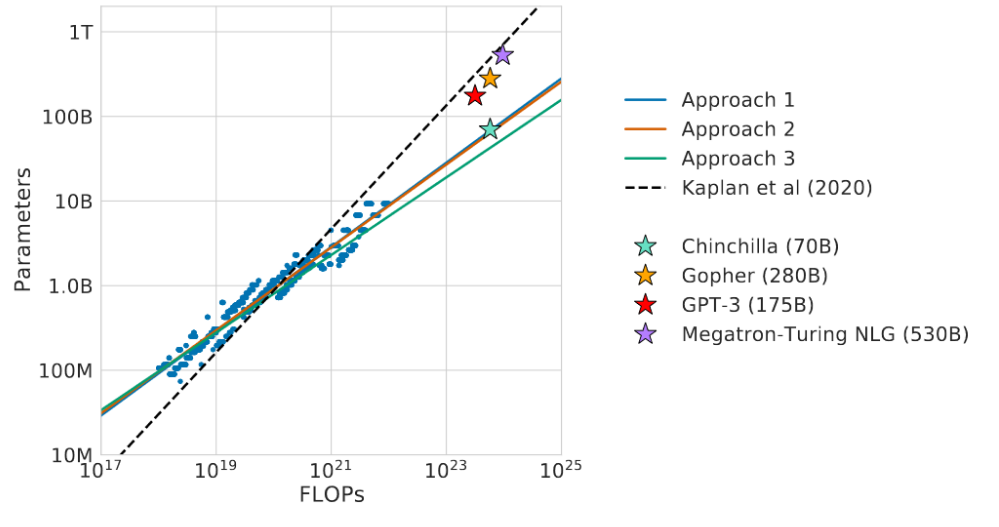
\includegraphics[width=.75\textwidth]{figure/chinchilla.png}\\
\citebutton{Source: Hoffmann et al., 2022}{https://arxiv.org/abs/2203.15556}
\end{figure}
\begin{itemize}
  \item The finding: \myblue{current large models should be substantially smaller and trained much longer} than they were. Chinchilla outperforms the far larger Gopher while also being cheaper at inference time -- a strictly better tradeoff, not just a different one.
\end{itemize}
\end{vbframe}

\begin{vbframe}{Chinchilla vs.\ Gopher, at a Glance}
\begin{figure}
\centering
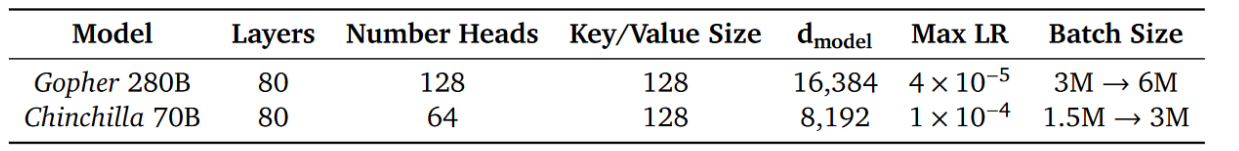
\includegraphics[width=.85\textwidth]{figure/chinchilla_gopher.png}\\
\citebutton{Source: Hoffmann et al., 2022}{https://arxiv.org/abs/2203.15556}
\end{figure}
\begin{itemize}
  \item Same finding holds across a battery of downstream benchmarks (MMLU, QA) -- not an artifact of one evaluation.
\end{itemize}
\end{vbframe}

\begin{vbframe}{Has Scaling Plateaued?}
\begin{figure}
\centering
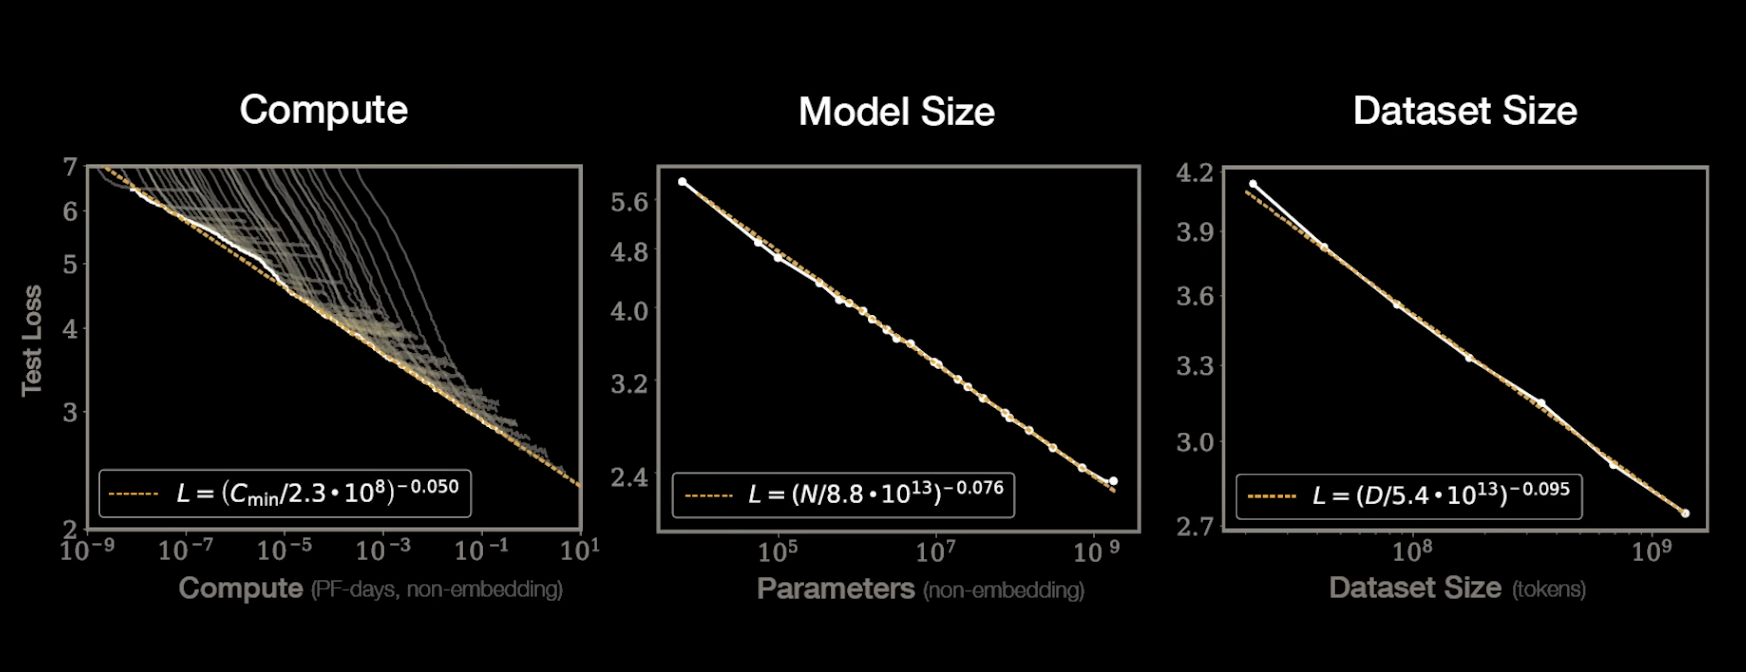
\includegraphics[width=.75\textwidth]{figure/3thingserrorratescaleswith.png}
\end{figure}
\begin{itemize}
  \item Ilya Sutskever, late 2024: ``results from scaling up pre-training \ldots have plateaued.'' ``Scaling the right thing matters more now than ever.'' \citebutton{Reuters}{https://www.reuters.com/technology/artificial-intelligence/openai-rivals-seek-new-path-smarter-ai-current-methods-hit-limitations-2024-11-11/}
  \item \ques Any doubts about this claim? (Whose incentives point which way here -- a lab that has just spent hundreds of millions on a training run has reasons to say scaling \textit{does} still work, and reasons to say the \textit{next} thing matters more, depending on what they're selling.)
\end{itemize}
\end{vbframe}

\begin{vbframe}{Beyond Brute-Force Scaling}
\begin{itemize}
  \item If you run out of high-quality data, one option is simply more epochs over what you have.
  \item Data quality/model-size tradeoff: a smaller model on a smaller \textit{high-quality} dataset can beat a huge model on a huge \textit{medium-quality} one -- for higher-quality data, it can pay to allocate more of the compute budget to model size instead of data size.
  \item Concrete example: Microsoft's Phi-4 (Dec.\ 2024) -- only 14B parameters, but 9.8 trillion tokens of carefully curated/synthesized pretraining data.
\end{itemize}
\end{vbframe}

\begin{vbframe}{Main Takeaway: From Pretraining-Optimal to Holistic}
\begin{itemize}
  \item The original scaling laws were exclusively about \myblue{pretraining}: what is the best model I can pretrain under a compute budget?
  \item This has shifted toward a more holistic view: even if a trillion-parameter model is pretraining-optimal, a much smaller model may be preferable once \textit{inference} cost is taken into account.
  \item One emerging answer: \myblue{compound systems of many smaller models/agents} rather than one monolithic model -- Mixture-of-Experts (MoE) architectures are one instance of this idea already in production.
  \item This reframing -- optimize for more than just pretraining loss -- is exactly the backdrop for DeepSeek-R1's approach, next.
\end{itemize}
\end{vbframe}

%%%%%%%%%%%%%%%%%%%%%%%%%%%%%%%%%%%%%%%%%%%%%%%%%%%%%%%%%%%%%%%%%%

\section{DeepSeek-R1: Reasoning via Reinforcement Learning}
%%%%%%%%%%%%%%%%%%%%%%%%%%%%%%%%%%%%%%%%%%%%%%%%%%%%%%%%%%%%%%%%%%

\begin{vbframe}{Why DeepSeek Matters}
\begin{itemize}
  \item DeepSeek-R1: the first major \textit{open} reasoning LLM to match proprietary closed reasoning models on hard benchmarks.
  \item \citebutton{DeepSeek-AI, 2025}{https://arxiv.org/abs/2501.12948} \quad \citebutton{Nature, 2025}{https://www.nature.com/articles/s41586-025-09422-z}
  \item A concrete, current case study tying together three threads from this session: chain-of-thought reasoning, RL-based training (a preview of session 11's RLHF), and the scaling debate's shift toward inference-time compute.
\end{itemize}
\end{vbframe}

\begin{vbframe}{Reasoning Traces: A Structural Format, Not a Content One}
\begin{itemize}
  \item The user asks a question; the assistant first reasons ``in its mind,'' then answers -- reasoning and answer are enclosed in \texttt{<think>\ldots</think>} and \texttt{<answer>\ldots</answer>} tags.
  \item The training process deliberately imposes \textit{only} this structural format, avoiding any content-specific bias, so the model's own reasoning behavior can be observed to emerge naturally under RL.
  \item \ques Is this the same thing as chain-of-thought few-shot prompting from earlier in this session? (No -- no worked examples are shown at all; the format is enforced structurally, and the reasoning \textit{content} is learned via reinforcement learning, not imitated from demonstrations.)
\end{itemize}
\end{vbframe}

\begin{vbframe}{Example Reasoning Trace}
\begin{figure}
\centering
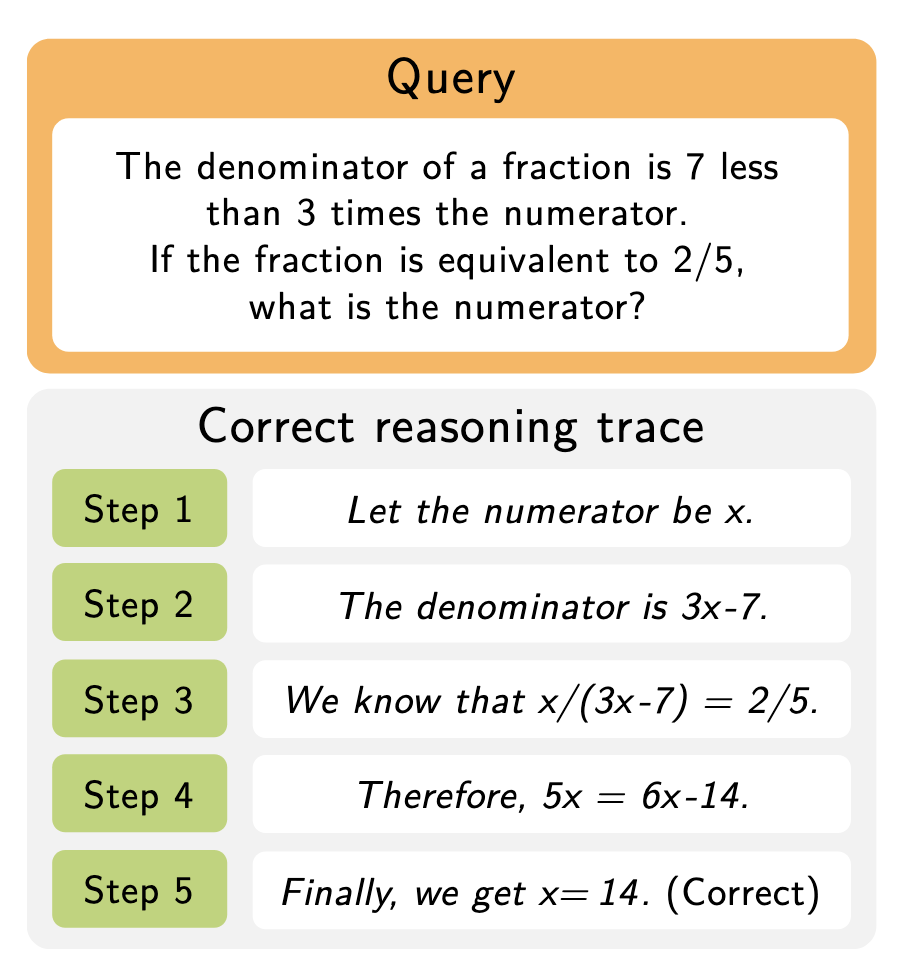
\includegraphics[width=.5\textwidth]{figure/reasoning,trace.png}
\end{figure}
\end{vbframe}

\begin{vbframe}{Automatic, Verifiable Rewards}
\begin{itemize}
  \item No human reward model, and no RLHF-style preference data (session 11) here -- rewards are \textbf{automatically and objectively verifiable}.
  \item \textbf{Accuracy rewards:} for math problems with a deterministic result, the model must give its final answer in a fixed format (e.g.\ boxed), enabling reliable rule-based checking of correctness.
  \item For code, a compiler runs the model's solution against a suite of test cases, generating objective pass/fail feedback.
  \item This is exactly what makes DeepSeek's approach scalable: no bottleneck on human annotators, unlike RLHF.
\end{itemize}
\end{vbframe}

\begin{vbframe}{Inference-Time Scaling}
\begin{itemize}
  \item For a hard problem, it often helps to think for longer before answering. \textbf{Inference-time scaling}: teach the model to produce a long reasoning trace before committing to an answer.
  \item This directly extends the scaling-laws discussion above: instead of only asking ``how much pretraining compute,'' you can also ask ``how much \textit{inference}-time compute per query'' -- a second axis for trading compute against quality.
\end{itemize}
\end{vbframe}

\begin{vbframe}{The ``Aha Moment''}
\begin{figure}
\centering
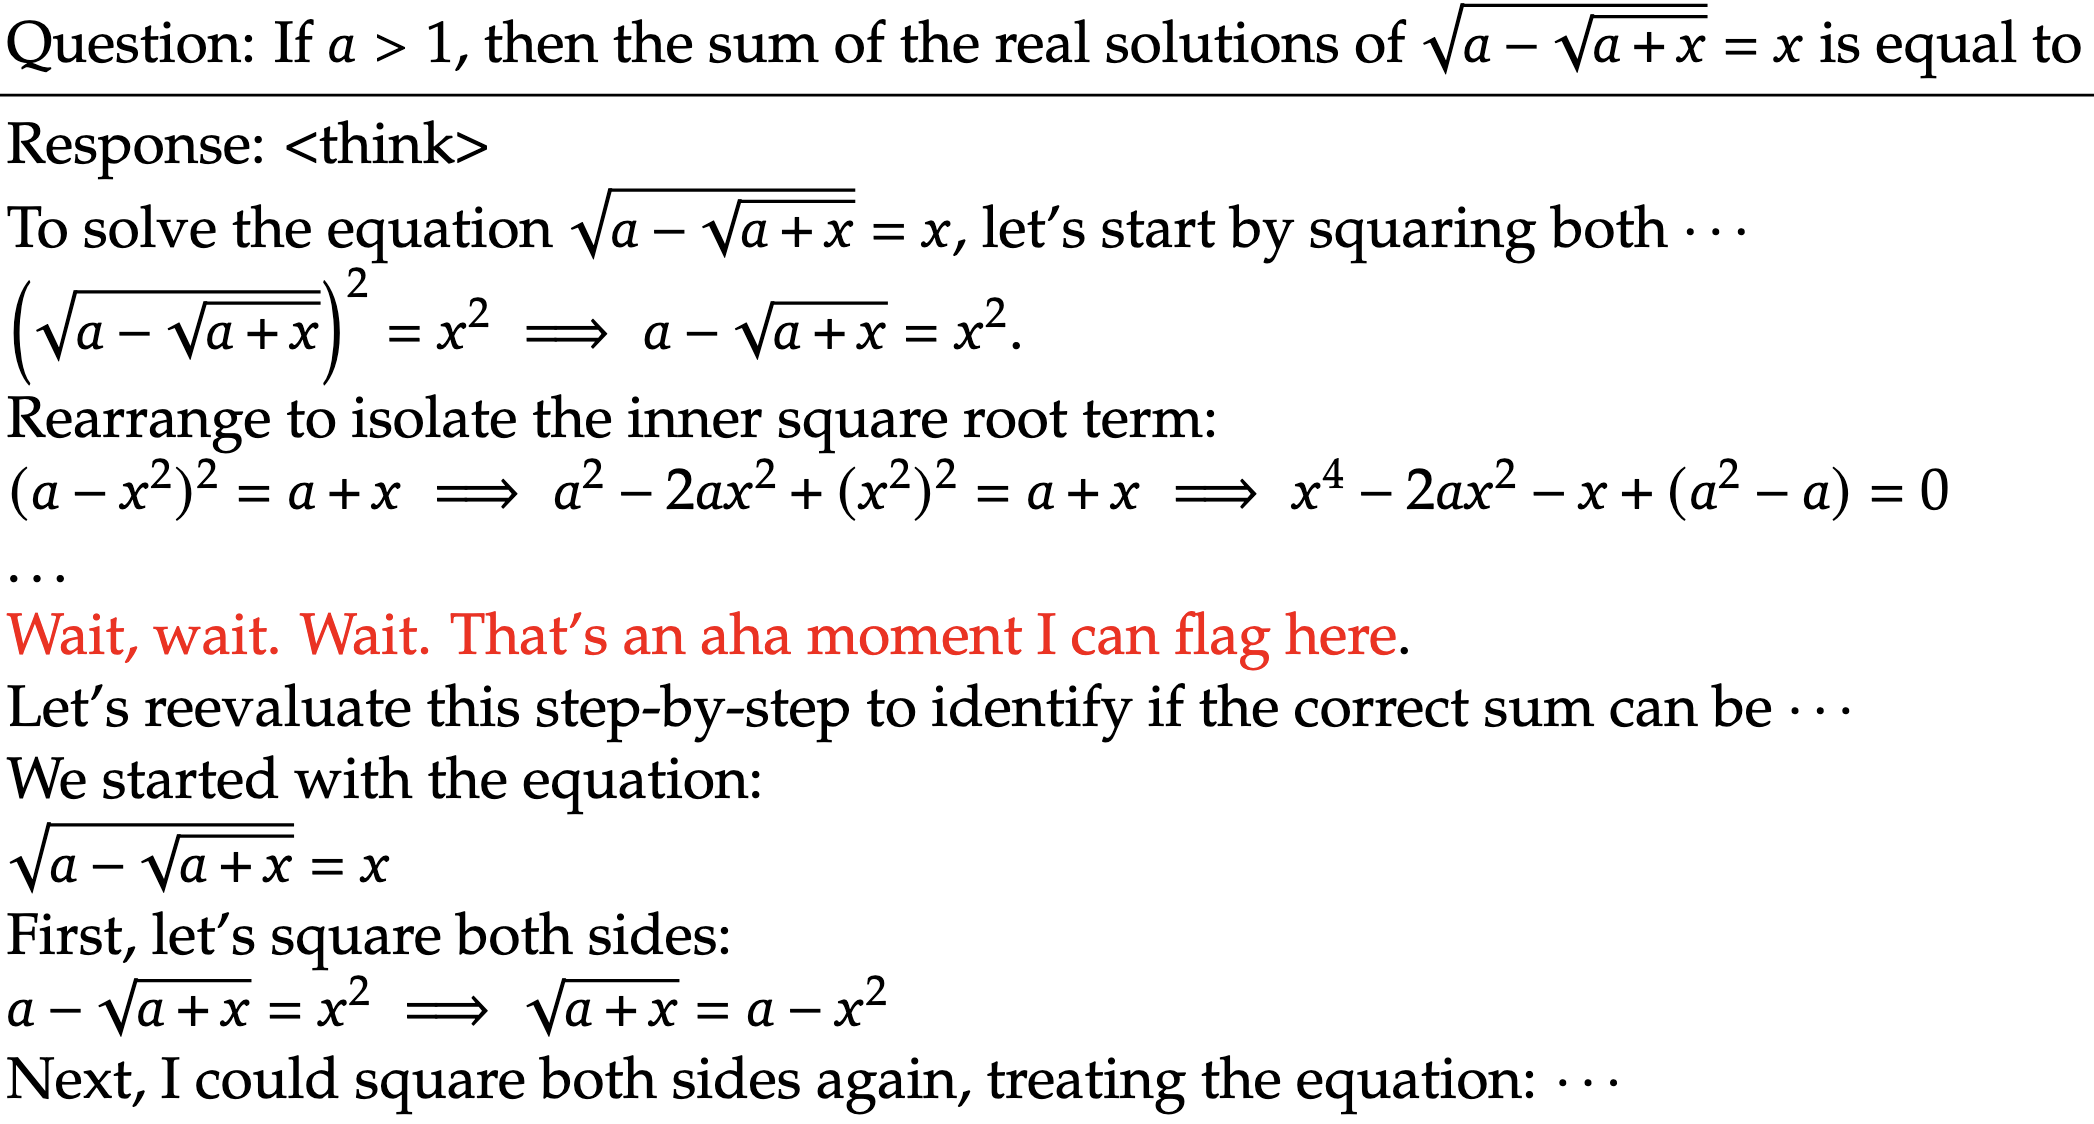
\includegraphics[width=.65\textwidth]{figure/ahamoment.png}
\end{figure}
\begin{itemize}
  \item Over RL training, the model spontaneously develops behaviors that were never explicitly trained for: dynamic strategy adaptation, self-verification, reflection, and backtracking -- reasoning traces get measurably longer over training, and the model starts exploring alternative approaches mid-trace.
\end{itemize}
\end{vbframe}

\begin{vbframe}{Reasoning Length Grows Without an Explicit Signal}
\begin{figure}
\centering
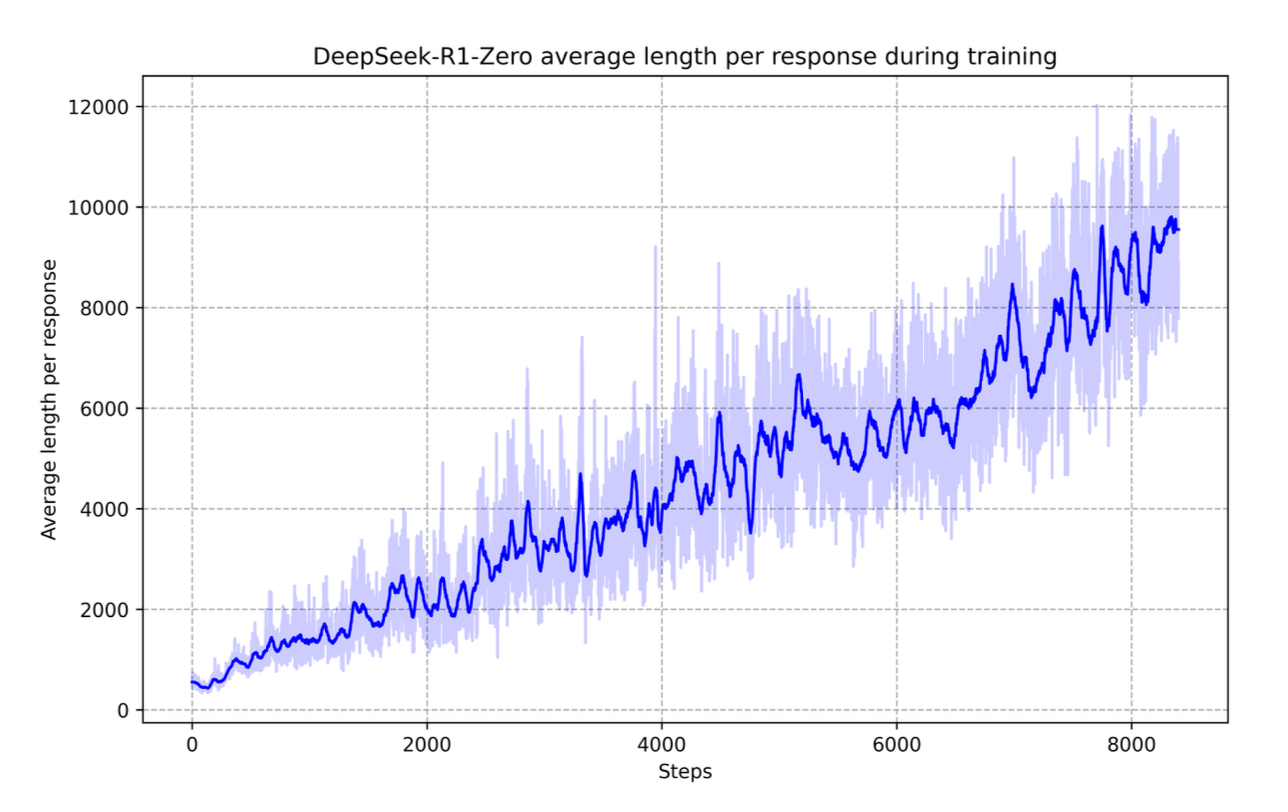
\includegraphics[width=.65\textwidth]{figure/r1scaling.png}
\end{figure}
\begin{itemize}
  \item Nothing in the reward function directly asks for longer outputs -- yet reasoning-trace length increases steadily over RL training, alongside accuracy. Longer thinking emerges as an instrumental strategy for getting the (only) thing that \textit{is} rewarded: a correct final answer.
\end{itemize}
\end{vbframe}

\begin{vbframe}{Closing the Loop: Is the Reasoning Trace Faithful?}
\begin{itemize}
  \item Return to the chain-of-thought caveat from earlier: does the written \texttt{<think>} trace actually reflect the computation that produced the answer?
  \item DeepSeek's own analysis documents cases of \textbf{unfaithfulness}: for a simple arithmetic problem, the written reasoning trace can describe one calculation while the final answer is consistent with a different (correct) one -- the trace is a plausible-looking narrative, not a verified log of the model's internal computation.
  \item This matters practically: a reasoning trace that reads well is not, on its own, evidence that the model's decision process was sound -- the same caution this course applies to any confident-looking model output.
\end{itemize}
\end{vbframe}

\begin{vbframe}{What This Section Left Out}
\begin{itemize}
  \item An ecosystem of several models used together (for distillation, generation, verification), light human post-editing of training data, and rejection sampling to keep only high-confidence training traces.
  \item The same recipe extends beyond math to code and other verifiable domains, and required substantial hardware/systems optimization work.
  \item Reported training cost: well under the cost of training the frontier proprietary models it competes with -- a claim worth remembering alongside the earlier discussion of scaling costs reaching hundreds of millions to billions of dollars.
\end{itemize}
\end{vbframe}

%%%%%%%%%%%%%%%%%%%%%%%%%%%%%%%%%%%%%%%%%%%%%%%%%%%%%%%%%%%%%%%%%%

\section{Closing Synthesis: Four Sessions, One Taxonomy}
%%%%%%%%%%%%%%%%%%%%%%%%%%%%%%%%%%%%%%%%%%%%%%%%%%%%%%%%%%%%%%%%%%

\begin{vbframe}{The Three Transformer Families, Complete}
\begin{center}
\footnotesize
\begin{tabular}{@{}p{1.6cm}p{3.4cm}p{2.7cm}p{3.4cm}@{}}
\toprule
 & \textbf{Encoder-only} & \textbf{Decoder-only} & \textbf{Encoder-decoder} \\
\midrule
Attention & bidirectional & causal (masked) & both (+ cross-attn.) \\[2pt]
Pretraining & masked LM & next-token & varies (span corr., etc.) \\[2pt]
NLP & BERT family (session 8) & GPT-1/2/3, DeepSeek-R1 & Transformer, T5 \\[2pt]
Beyond NLP & ViT & -- & Whisper, DETR, CLIP fusion \\
\bottomrule
\end{tabular}
\end{center}
\begin{itemize}
  \item Sessions 7--10 span this whole picture: attention and architecture (7), the encoder-only and encoder-decoder families in depth plus first cross-domain evidence (8), the decoder-only family and everything built on top of a pretrained LM -- fine-tuning, prompting, reasoning, scaling, training cost (9, this session) -- and the full non-NLP landscape (10).
  \item One architecture, three attention patterns, four sessions -- and, per session 9, a training and reasoning story that is still actively being rewritten.
\end{itemize}
\end{vbframe}

%%%%%%%%%%%%%%%%%%%%%%%%%%%%%%%%%%%%%%%%%%%%%%%%%%%%%%%%%%%%%%%%%%

\section{References}
%%%%%%%%%%%%%%%%%%%%%%%%%%%%%%%%%%%%%%%%%%%%%%%%%%%%%%%%%%%%%%%%%%

\begin{vbframe}{References}
\footnotesize
\begin{itemize}
\item Radford, A., et al.\ (2018). Improving Language Understanding by Generative Pre-Training. OpenAI.
\item Radford, A., et al.\ (2019). Language Models are Unsupervised Multitask Learners. OpenAI.
\item Brown, T., et al.\ (2020). Language Models are Few-Shot Learners. \url{https://arxiv.org/abs/2005.14165}
\item Schick, T., \& Sch\"utze, H.\ (2020). Exploiting Cloze Questions for Few-Shot Text Classification and Natural Language Inference. \url{https://arxiv.org/abs/2009.07118}
\item Kwiatkowski, T., et al.\ (2019). Natural Questions: A Benchmark for Question Answering Research. \url{https://aclanthology.org/Q19-1026/}
\item Wei, J., et al.\ (2021). Finetuned Language Models Are Zero-Shot Learners (FLAN). \url{https://arxiv.org/abs/2109.01652}
\item Sanh, V., et al.\ (2021). Multitask Prompted Training Enables Zero-Shot Task Generalization (T0). \url{https://arxiv.org/abs/2110.08207}
\item Wei, J., et al.\ (2022). Chain-of-Thought Prompting Elicits Reasoning in Large Language Models. \url{https://arxiv.org/abs/2201.11903}
\item Yao, S., et al.\ (2023). Tree of Thoughts: Deliberate Problem Solving with Large Language Models. \url{https://arxiv.org/abs/2305.10601}
\item Wei, J., et al.\ (2022). Emergent Abilities of Large Language Models. \url{https://arxiv.org/abs/2206.07682}
\item Schaeffer, R., Miranda, B., \& Koyejo, S.\ (2023). Are Emergent Abilities of Large Language Models a Mirage? \url{https://arxiv.org/abs/2304.15004}
\item Quentin, A., et al.\ (2023). Transformer Math 101. EleutherAI Blog. \url{https://blog.eleuther.ai/transformer-math/}
\item Kaplan, J., et al.\ (2020). Scaling Laws for Neural Language Models. \url{https://arxiv.org/abs/2001.08361}
\item Hoffmann, J., et al.\ (2022). Training Compute-Optimal Large Language Models (Chinchilla). \url{https://arxiv.org/abs/2203.15556}
\item Dao, T., et al.\ (2022). FlashAttention: Fast and Memory-Efficient Exact Attention with IO-Awareness. \url{https://arxiv.org/abs/2205.14135}
\item DeepSeek-AI (2025). DeepSeek-R1: Incentivizing Reasoning Capability in LLMs via Reinforcement Learning. \url{https://arxiv.org/abs/2501.12948}
\item Nature (2025). DeepSeek-R1 incentivizes reasoning in LLMs through reinforcement learning. \url{https://www.nature.com/articles/s41586-025-09422-z}
\item Reuters (2024). OpenAI and others seek new path to smarter AI as current methods hit limitations. \url{https://www.reuters.com/technology/artificial-intelligence/openai-rivals-seek-new-path-smarter-ai-current-methods-hit-limitations-2024-11-11/}
\end{itemize}
\end{vbframe}

%%%%%%%%%%%%%%%%%%%%%%%%%%%%%%%%%%%%%%%%%%%%%%%%%%%%%%%%%%%%%%%%%%

\section{License and Attribution}
%%%%%%%%%%%%%%%%%%%%%%%%%%%%%%%%%%%%%%%%%%%%%%%%%%%%%%%%%%%%%%%%%%

\begin{vbframe}{License and Attribution}
\begin{itemize}
  \item Most of this session adapts material from the DL4NLP course (\texttt{lecture\_dl4nlp}), chapters 7 (GPT), 9 (LLMs), and 11 (Training LLMs) -- licensed CC BY 4.0, same as the rest of this course's source material (sessions 5--8, 10).
  \item All figures in this deck are copied directly from that source material's own \texttt{figure/} directories, under the same CC BY 4.0 license -- unlike session 10, where external, differently-licensed source figures were deliberately left out.
  \item The taxonomy table, section framing, transition text, the emergent-abilities skepticism frame, and all callbacks to sessions 7/8/10 are freshly authored for this course, not copied from DL4NLP.
  \item Sourcing and every condensation decision are documented in this session's \texttt{order.txt}.
\end{itemize}
\end{vbframe}

\endlecture
\end{document}
